% Generated by Sphinx.
\def\sphinxdocclass{report}
\documentclass[a4paper,10pt,english]{sphinxmanual}
\usepackage[utf8]{inputenc}
\DeclareUnicodeCharacter{00A0}{\nobreakspace}
\usepackage[T1]{fontenc}
\usepackage{babel}
\usepackage{times}
\usepackage[Bjarne]{fncychap}
\usepackage{longtable}
\usepackage{sphinx}
\usepackage{multirow}


\title{MapClass Documentation}
\date{September 10, 2012}
\release{0.1.0}
\author{Christof Buchbender}
\newcommand{\sphinxlogo}{}
\renewcommand{\releasename}{Release}
\makeindex

\makeatletter
\def\PYG@reset{\let\PYG@it=\relax \let\PYG@bf=\relax%
    \let\PYG@ul=\relax \let\PYG@tc=\relax%
    \let\PYG@bc=\relax \let\PYG@ff=\relax}
\def\PYG@tok#1{\csname PYG@tok@#1\endcsname}
\def\PYG@toks#1+{\ifx\relax#1\empty\else%
    \PYG@tok{#1}\expandafter\PYG@toks\fi}
\def\PYG@do#1{\PYG@bc{\PYG@tc{\PYG@ul{%
    \PYG@it{\PYG@bf{\PYG@ff{#1}}}}}}}
\def\PYG#1#2{\PYG@reset\PYG@toks#1+\relax+\PYG@do{#2}}

\def\PYG@tok@gd{\def\PYG@tc##1{\textcolor[rgb]{0.63,0.00,0.00}{##1}}}
\def\PYG@tok@gu{\let\PYG@bf=\textbf\def\PYG@tc##1{\textcolor[rgb]{0.50,0.00,0.50}{##1}}}
\def\PYG@tok@gt{\def\PYG@tc##1{\textcolor[rgb]{0.00,0.25,0.82}{##1}}}
\def\PYG@tok@gs{\let\PYG@bf=\textbf}
\def\PYG@tok@gr{\def\PYG@tc##1{\textcolor[rgb]{1.00,0.00,0.00}{##1}}}
\def\PYG@tok@cm{\let\PYG@it=\textit\def\PYG@tc##1{\textcolor[rgb]{0.25,0.50,0.56}{##1}}}
\def\PYG@tok@vg{\def\PYG@tc##1{\textcolor[rgb]{0.73,0.38,0.84}{##1}}}
\def\PYG@tok@m{\def\PYG@tc##1{\textcolor[rgb]{0.13,0.50,0.31}{##1}}}
\def\PYG@tok@mh{\def\PYG@tc##1{\textcolor[rgb]{0.13,0.50,0.31}{##1}}}
\def\PYG@tok@cs{\def\PYG@tc##1{\textcolor[rgb]{0.25,0.50,0.56}{##1}}\def\PYG@bc##1{\colorbox[rgb]{1.00,0.94,0.94}{##1}}}
\def\PYG@tok@ge{\let\PYG@it=\textit}
\def\PYG@tok@vc{\def\PYG@tc##1{\textcolor[rgb]{0.73,0.38,0.84}{##1}}}
\def\PYG@tok@il{\def\PYG@tc##1{\textcolor[rgb]{0.13,0.50,0.31}{##1}}}
\def\PYG@tok@go{\def\PYG@tc##1{\textcolor[rgb]{0.19,0.19,0.19}{##1}}}
\def\PYG@tok@cp{\def\PYG@tc##1{\textcolor[rgb]{0.00,0.44,0.13}{##1}}}
\def\PYG@tok@gi{\def\PYG@tc##1{\textcolor[rgb]{0.00,0.63,0.00}{##1}}}
\def\PYG@tok@gh{\let\PYG@bf=\textbf\def\PYG@tc##1{\textcolor[rgb]{0.00,0.00,0.50}{##1}}}
\def\PYG@tok@ni{\let\PYG@bf=\textbf\def\PYG@tc##1{\textcolor[rgb]{0.84,0.33,0.22}{##1}}}
\def\PYG@tok@nl{\let\PYG@bf=\textbf\def\PYG@tc##1{\textcolor[rgb]{0.00,0.13,0.44}{##1}}}
\def\PYG@tok@nn{\let\PYG@bf=\textbf\def\PYG@tc##1{\textcolor[rgb]{0.05,0.52,0.71}{##1}}}
\def\PYG@tok@no{\def\PYG@tc##1{\textcolor[rgb]{0.38,0.68,0.84}{##1}}}
\def\PYG@tok@na{\def\PYG@tc##1{\textcolor[rgb]{0.25,0.44,0.63}{##1}}}
\def\PYG@tok@nb{\def\PYG@tc##1{\textcolor[rgb]{0.00,0.44,0.13}{##1}}}
\def\PYG@tok@nc{\let\PYG@bf=\textbf\def\PYG@tc##1{\textcolor[rgb]{0.05,0.52,0.71}{##1}}}
\def\PYG@tok@nd{\let\PYG@bf=\textbf\def\PYG@tc##1{\textcolor[rgb]{0.33,0.33,0.33}{##1}}}
\def\PYG@tok@ne{\def\PYG@tc##1{\textcolor[rgb]{0.00,0.44,0.13}{##1}}}
\def\PYG@tok@nf{\def\PYG@tc##1{\textcolor[rgb]{0.02,0.16,0.49}{##1}}}
\def\PYG@tok@si{\let\PYG@it=\textit\def\PYG@tc##1{\textcolor[rgb]{0.44,0.63,0.82}{##1}}}
\def\PYG@tok@s2{\def\PYG@tc##1{\textcolor[rgb]{0.25,0.44,0.63}{##1}}}
\def\PYG@tok@vi{\def\PYG@tc##1{\textcolor[rgb]{0.73,0.38,0.84}{##1}}}
\def\PYG@tok@nt{\let\PYG@bf=\textbf\def\PYG@tc##1{\textcolor[rgb]{0.02,0.16,0.45}{##1}}}
\def\PYG@tok@nv{\def\PYG@tc##1{\textcolor[rgb]{0.73,0.38,0.84}{##1}}}
\def\PYG@tok@s1{\def\PYG@tc##1{\textcolor[rgb]{0.25,0.44,0.63}{##1}}}
\def\PYG@tok@gp{\let\PYG@bf=\textbf\def\PYG@tc##1{\textcolor[rgb]{0.78,0.36,0.04}{##1}}}
\def\PYG@tok@sh{\def\PYG@tc##1{\textcolor[rgb]{0.25,0.44,0.63}{##1}}}
\def\PYG@tok@ow{\let\PYG@bf=\textbf\def\PYG@tc##1{\textcolor[rgb]{0.00,0.44,0.13}{##1}}}
\def\PYG@tok@sx{\def\PYG@tc##1{\textcolor[rgb]{0.78,0.36,0.04}{##1}}}
\def\PYG@tok@bp{\def\PYG@tc##1{\textcolor[rgb]{0.00,0.44,0.13}{##1}}}
\def\PYG@tok@c1{\let\PYG@it=\textit\def\PYG@tc##1{\textcolor[rgb]{0.25,0.50,0.56}{##1}}}
\def\PYG@tok@kc{\let\PYG@bf=\textbf\def\PYG@tc##1{\textcolor[rgb]{0.00,0.44,0.13}{##1}}}
\def\PYG@tok@c{\let\PYG@it=\textit\def\PYG@tc##1{\textcolor[rgb]{0.25,0.50,0.56}{##1}}}
\def\PYG@tok@mf{\def\PYG@tc##1{\textcolor[rgb]{0.13,0.50,0.31}{##1}}}
\def\PYG@tok@err{\def\PYG@bc##1{\fcolorbox[rgb]{1.00,0.00,0.00}{1,1,1}{##1}}}
\def\PYG@tok@kd{\let\PYG@bf=\textbf\def\PYG@tc##1{\textcolor[rgb]{0.00,0.44,0.13}{##1}}}
\def\PYG@tok@ss{\def\PYG@tc##1{\textcolor[rgb]{0.32,0.47,0.09}{##1}}}
\def\PYG@tok@sr{\def\PYG@tc##1{\textcolor[rgb]{0.14,0.33,0.53}{##1}}}
\def\PYG@tok@mo{\def\PYG@tc##1{\textcolor[rgb]{0.13,0.50,0.31}{##1}}}
\def\PYG@tok@mi{\def\PYG@tc##1{\textcolor[rgb]{0.13,0.50,0.31}{##1}}}
\def\PYG@tok@kn{\let\PYG@bf=\textbf\def\PYG@tc##1{\textcolor[rgb]{0.00,0.44,0.13}{##1}}}
\def\PYG@tok@o{\def\PYG@tc##1{\textcolor[rgb]{0.40,0.40,0.40}{##1}}}
\def\PYG@tok@kr{\let\PYG@bf=\textbf\def\PYG@tc##1{\textcolor[rgb]{0.00,0.44,0.13}{##1}}}
\def\PYG@tok@s{\def\PYG@tc##1{\textcolor[rgb]{0.25,0.44,0.63}{##1}}}
\def\PYG@tok@kp{\def\PYG@tc##1{\textcolor[rgb]{0.00,0.44,0.13}{##1}}}
\def\PYG@tok@w{\def\PYG@tc##1{\textcolor[rgb]{0.73,0.73,0.73}{##1}}}
\def\PYG@tok@kt{\def\PYG@tc##1{\textcolor[rgb]{0.56,0.13,0.00}{##1}}}
\def\PYG@tok@sc{\def\PYG@tc##1{\textcolor[rgb]{0.25,0.44,0.63}{##1}}}
\def\PYG@tok@sb{\def\PYG@tc##1{\textcolor[rgb]{0.25,0.44,0.63}{##1}}}
\def\PYG@tok@k{\let\PYG@bf=\textbf\def\PYG@tc##1{\textcolor[rgb]{0.00,0.44,0.13}{##1}}}
\def\PYG@tok@se{\let\PYG@bf=\textbf\def\PYG@tc##1{\textcolor[rgb]{0.25,0.44,0.63}{##1}}}
\def\PYG@tok@sd{\let\PYG@it=\textit\def\PYG@tc##1{\textcolor[rgb]{0.25,0.44,0.63}{##1}}}

\def\PYGZbs{\char`\\}
\def\PYGZus{\char`\_}
\def\PYGZob{\char`\{}
\def\PYGZcb{\char`\}}
\def\PYGZca{\char`\^}
\def\PYGZsh{\char`\#}
\def\PYGZpc{\char`\%}
\def\PYGZdl{\char`\$}
\def\PYGZti{\char`\~}
% for compatibility with earlier versions
\def\PYGZat{@}
\def\PYGZlb{[}
\def\PYGZrb{]}
\makeatother

\begin{document}

\maketitle
\tableofcontents
\phantomsection\label{index::doc}


Astrolyze is a python-package with several functions for reduction and analysis
of (mainly) radioastronomical data analysis. It developed over the course of
my Diploma and PhD thesis. I decided to package the functions because I think
that they may be usefull to other astronomers. The package is open for
colaboration.


\chapter{Installation of astrolyze}
\label{installation::doc}\label{installation:astrolyze-documentation}\label{installation:installation-of-astrolyze}
The installation of astrolyze is done via:

\begin{Verbatim}[commandchars=\\\{\}]
sudo python setup.py install
\end{Verbatim}

So far there are no options for the installation path. The setup.py script will
generate a \code{\textasciitilde{}/.astrolyze} folder in the home account of the user.  This
folder is needed to store a database in \code{\textasciitilde{}/.astrolyze/database/parameters.db}
containing parameters of the sources, lines, and instruments used.

Using the {\color{red}\bfseries{}{}`Naming Convention{}`\_} astrolyze attempts to read this database when
opening a map or spectrum to obtain additional information. Please see
{\color{red}\bfseries{}{}`Parameter Database{}`\_} for more details.


\chapter{Manual}
\label{manual:manual}\label{manual::doc}
This tutorial explains how astrolyze can be used to ease reduction,
analysis and modification of (radio-)astronomical data and images.


\bigskip\hrule{}\bigskip



\section{Motivation}
\label{manual:motivation}
First, before we delve into the details, let me give some examples of what
astrolyze is capable of, so that you can decide if it could be of use for you.
This is a snapshot of the most powerful functions of astrolyze; a thorough
introduction with more features and possibilities follows below.


\subsection{Inter-operating Fits, Gildas and Miriad}
\label{manual:inter-operating-fits-gildas-and-miriad}
Using the astrolyze package it is possible to use different file formats and
different programs from within python seamlessly. Say, for the sake of
demonstrations, that you have a Fits image called
\code{M33\_30m\_12CO10\_Tmb\_12.fits} and that you want to smooth it in miriad to 40
arcsec resolution, re-project it with Gildas to a new central coordinate and
finally convert it back to fits-format:

This is how you would do it with astrolyze:

\begin{Verbatim}[commandchars=\\\{\}]
\PYG{k+kn}{from} \PYG{n+nn}{astrolyze} \PYG{k+kn}{import} \PYG{o}{*}
\PYG{n}{map\PYGZus{}} \PYG{o}{=} \PYG{n}{FitsMap}\PYG{p}{(}\PYG{l+s}{'}\PYG{l+s}{M33\PYGZus{}30m\PYGZus{}12CO10\PYGZus{}Tmb\PYGZus{}12.fits}\PYG{l+s}{'}\PYG{p}{)}
\PYG{n}{map\PYGZus{}} \PYG{o}{=} \PYG{n}{map\PYGZus{}}\PYG{o}{.}\PYG{n}{toMiriad}\PYG{p}{(}\PYG{p}{)}
\PYG{n}{map\PYGZus{}} \PYG{o}{=} \PYG{n}{map\PYGZus{}}\PYG{o}{.}\PYG{n}{smooth}\PYG{p}{(}\PYG{l+m+mi}{40}\PYG{p}{)}
\PYG{n}{map\PYGZus{}} \PYG{o}{=} \PYG{n}{map\PYGZus{}}\PYG{o}{.}\PYG{n}{toGildas}\PYG{p}{(}\PYG{p}{)}
\PYG{n}{map\PYGZus{}} \PYG{o}{=} \PYG{n}{map\PYGZus{}}\PYG{o}{.}\PYG{n}{reproject}\PYG{p}{(}\PYG{n}{coordinate}\PYG{o}{=}\PYG{p}{[}\PYG{l+s}{'}\PYG{l+s}{01:34:50.890}\PYG{l+s}{'}\PYG{p}{,} \PYG{l+s}{'}\PYG{l+s}{+31:08:28.03}\PYG{l+s}{'}\PYG{p}{]}\PYG{p}{)}
\PYG{n}{map\PYGZus{}} \PYG{o}{=} \PYG{n}{map\PYGZus{}}\PYG{o}{.}\PYG{n}{toFits}\PYG{p}{(}\PYG{p}{)}
\end{Verbatim}

Please note the special format of the map name. The format follows a certain
\code{naming convention} that has to be used with astrolyze. The reason for the
naming conventions and it's internal logic is explained below.

As a side note I use an underscore for the \code{map\_} variable, because
otherwise the python function \code{map} is overwritten which may lead to problems.


\subsection{Changing map units}
\label{manual:changing-map-units}
With astrolyze the units of a map can be quickly transformed between common
units used in (Radio-) Astronomy (as far as the conversion was implemented
already). Take for example again the \code{M33\_30m\_12CO10\_Tmb\_12.fits} map.
Following the naming convention this map is in main beam temperature
(Tmb). Changing its units to \code{JyB} is as easy as:

\begin{Verbatim}[commandchars=\\\{\}]
\PYG{k+kn}{from} \PYG{n+nn}{astrolyze} \PYG{k+kn}{import} \PYG{o}{*}
\PYG{n}{map\PYGZus{}} \PYG{o}{=} \PYG{n}{FitsMap}\PYG{p}{(}\PYG{l+s}{'}\PYG{l+s}{M33\PYGZus{}30m\PYGZus{}12CO10\PYGZus{}Tmb\PYGZus{}12.fits}\PYG{l+s}{'}\PYG{p}{)}
\PYG{n}{map\PYGZus{}} \PYG{o}{=} \PYG{n}{map\PYGZus{}}\PYG{o}{.}\PYG{n}{change\PYGZus{}unit}\PYG{p}{(}\PYG{l+s}{'}\PYG{l+s}{JyB}\PYG{l+s}{'}\PYG{p}{)}
\end{Verbatim}

Another side note: It's only that easy when astrolyze is set-up
correctly as described in TODO. Link to Installation.  Also please check the
results for plausibility in case there are faults in the interal conversion
algorithms.


\subsection{Working with stacks of images}
\label{manual:working-with-stacks-of-images}
The previous examples show the principles how a single map can be treated in
astrolyze. However the package also includes a way to work on a stack of images
and perform tasks on all of them.

To create a stack, all files that are going to be in the stack have to be
located in one folder (with possible sub-folders NOTE: The functionality with
sub-folders are is however not thoroughly tested however.)
A stack is initialized as follows:

\begin{Verbatim}[commandchars=\\\{\}]
\PYG{k+kn}{from} \PYG{n+nn}{astrolyze} \PYG{k+kn}{import} \PYG{o}{*}
\PYG{n}{example\PYGZus{}stack} \PYG{o}{=} \PYG{n}{Stack}\PYG{p}{(}\PYG{l+s}{'}\PYG{l+s}{path\PYGZus{}to\PYGZus{}folder}\PYG{l+s}{'}\PYG{p}{)}
\end{Verbatim}

The maps can be a mix of GILDAS, Fits and MIRIAD maps. The Instance of the
Stack object (here: \code{example\_stack}) contains a variable called stack which
is a list with Instances of the corresponding maps Objects (GildasMap, FitsMap
and MiriadMap).

The stack module provides several tools to \code{unify} the stack for further
analysis. The maps can be all re-gridded and re-projected to the same central
coordinates, pixel-sizes and dimensions as a given template image via:

\begin{Verbatim}[commandchars=\\\{\}]
\PYG{n}{example\PYGZus{}stack}\PYG{o}{.}\PYG{n}{unify\PYGZus{}dimensions}\PYG{p}{(}\PYG{n}{template}\PYG{o}{=}\PYG{l+s}{'}\PYG{l+s}{path\PYGZus{}to\PYGZus{}template\PYGZus{}file}\PYG{l+s}{'}\PYG{p}{,}
                                \PYG{n}{folder}\PYG{o}{=}\PYG{l+s}{'}\PYG{l+s}{path\PYGZus{}to\PYGZus{}output\PYGZus{}folder}\PYG{l+s}{'}\PYG{p}{)}
\end{Verbatim}

Also the maps can be all smoothed to the same resolution, by default this is
the largest resolution found in the stack but can also be given manually:

\begin{Verbatim}[commandchars=\\\{\}]
\PYG{n}{example\PYGZus{}stack}\PYG{o}{.}\PYG{n}{unify\PYGZus{}resolution}\PYG{p}{(}\PYG{n}{folder}\PYG{o}{=}\PYG{l+s}{'}\PYG{l+s}{path\PYGZus{}to\PYGZus{}output\PYGZus{}folder}\PYG{l+s}{'}\PYG{p}{)}
\end{Verbatim}

Astrolyze includes also some unit conversions that can be used to change all
maps to the same resolutions as long as the input and output units are
programmed. See (TODO) for more details. For the stack:

\begin{Verbatim}[commandchars=\\\{\}]
\PYG{n}{example\PYGZus{}stack}\PYG{o}{.}\PYG{n}{unify\PYGZus{}units}\PYG{p}{(}\PYG{n}{folder}\PYG{o}{=}\PYG{l+s}{'}\PYG{l+s}{path\PYGZus{}to\PYGZus{}output\PYGZus{}folder}\PYG{l+s}{'}\PYG{p}{)}
\end{Verbatim}

can be used.


\subsection{Producing SEDs}
\label{manual:producing-seds}
Build on-top of the stack module astrolyze also contains an \code{sed} module
which allows to analyze and plot dust-seds. The SEDs can be read out for an
arbitrary number of positions or for a full maps. In the latter case
temperature and mass maps will be created.

When all maps have the same resolution and dimension (i.e. pixel size and
number) producing temperature maps can be done as follows:

\begin{Verbatim}[commandchars=\\\{\}]
\PYG{k+kn}{from} \PYG{n+nn}{astrolyze} \PYG{k+kn}{import} \PYG{o}{*}
\PYG{n}{sed} \PYG{o}{=} \PYG{n}{SedStack}\PYG{p}{(}\PYG{n}{folder}\PYG{o}{=}\PYG{l+s}{'}\PYG{l+s}{path\PYGZus{}to\PYGZus{}input\PYGZus{}folder}\PYG{l+s}{'}\PYG{p}{,} \PYG{n}{full\PYGZus{}map}\PYG{o}{=}\PYG{n+nb+bp}{True}\PYG{p}{,}
               \PYG{n}{output\PYGZus{}folder}\PYG{o}{=}\PYG{l+s}{'}\PYG{l+s}{path\PYGZus{}to\PYGZus{}output\PYGZus{}folder}\PYG{l+s}{'}\PYG{p}{)}
\end{Verbatim}

To generate SEDs at given coordinates it is easiest to provide a separate file
(e.g. \code{coordinates.txt})with the names and coordinates of the positions to be
extracted as follows:

\begin{Verbatim}[commandchars=\\\{\}]
source\_1    1:34:7.00     +30:47:52.00
source\_2    1:33:55.80    +30:43:2.00
source\_3    1:33:52.40    +30:39:18.00
  .              .             .
  .              .             .
  .              .             .
\end{Verbatim}

Then a stack of seds can be created:

\begin{Verbatim}[commandchars=\\\{\}]
\PYG{k+kn}{from} \PYG{n+nn}{astrolyze} \PYG{k+kn}{import} \PYG{o}{*}
\PYG{n}{seds} \PYG{o}{=} \PYG{n}{SedStack}\PYG{p}{(}\PYG{n}{folder}\PYG{o}{=}\PYG{l+s}{'}\PYG{l+s}{path\PYGZus{}to\PYGZus{}input\PYGZus{}folder}\PYG{l+s}{'}\PYG{p}{,} \PYG{n}{flux\PYGZus{}acquisition}\PYG{o}{=}\PYG{l+s}{'}\PYG{l+s}{pixel}\PYG{l+s}{'}\PYG{p}{,}\PYG{p}{)}
\end{Verbatim}


\subsection{Not only images ...}
\label{manual:not-only-images}
Last but not least astrolyze is also able to work with 30m class spectra from
within python based on the same principles used to work with
images/maps. Implementation of this feature has however only started...


\bigskip\hrule{}\bigskip



\section{astrolyze}
\label{manual:astrolyze}
I started to develop astrolyze to be able to inter-operate the Programs PyFits,
MIRIAD and GILDAS. One reason was that the Gildas task are very
cumbersome to script and once scripted, the scripts are not very flexible. Also
there are some tasks in GILDAS that are (in my opinion) easier to use than in
miriad and vice versa, due to different sets of features.

However, the real power of astrolyze comes from it's internal tracking of
changes to the most important parameters of the maps (or spectral-files), which
are stored directly in the file-names, following a naming-convention.


\section{Naming Convention}
\label{manual:naming-convention}
A Name that follows the `Naming Convention' is for example:
\code{M33\_30m-HERA\_CO21\_Ta*\_12\_cube\_regrid.fits}

All items \textbf{MUST} be separated by an underscore (\_) and \textbf{HAVE} to include at
the following properties in the same order:
\begin{enumerate}
\item {} 
source

\item {} 
telescope

\item {} 
species (wavelength OR frequency OR line-name)

\item {} 
flux unit

\item {} 
resolution

\end{enumerate}

When opening a map with astrolyze these items are transferred to python
variables of the \emph{Map class} (see below).  All additional items
separated by underscores are treated as comments. Comments are not
transferred to individual internal variables of the map objects but are passed
on as a list to the single variable comments.

The last item is followed by the files extension:
\begin{itemize}
\item {} 
.fits -\textgreater{} FITS

\item {} 
.gdf, .mean, .velo, .width, .lmv -\textgreater{} GILDAS

\item {} 
nothing -\textgreater{} MIRIAD (Miriads file format uses directories to store the data.)

\end{itemize}

Maps that are not following this name convention are \textbf{not} supported. This is
to assure that all parts of the program work, since they strongly depend on the
parameters passed on by the file-name, as is explained in this tutorial or the
documentation of the functions.

Using the example file-name above, opening this file with astrolyze as follows:

\begin{Verbatim}[commandchars=\\\{\}]
\PYG{k+kn}{from} \PYG{n+nn}{astrolyze} \PYG{k+kn}{import} \PYG{o}{*}
\PYG{n}{map\PYGZus{}} \PYG{o}{=} \PYG{n}{FitsMap}\PYG{p}{(}\PYG{l+s}{'}\PYG{l+s}{M33\PYGZus{}30m\PYGZus{}12CO10\PYGZus{}Tmb\PYGZus{}12\PYGZus{}cube\PYGZus{}regrid.fits}\PYG{l+s}{'}\PYG{p}{)}
\end{Verbatim}

would generate the following python variables:

\begin{Verbatim}[commandchars=\\\{\}]
\PYG{n}{map\PYGZus{}}\PYG{o}{.}\PYG{n}{source} \PYG{o}{=} \PYG{l+s}{'}\PYG{l+s}{M33}\PYG{l+s}{'}
\PYG{n}{map\PYGZus{}}\PYG{o}{.}\PYG{n}{telescope} \PYG{o}{=} \PYG{l+s}{'}\PYG{l+s}{30m}\PYG{l+s}{'}
\PYG{n}{map\PYGZus{}}\PYG{o}{.}\PYG{n}{species} \PYG{o}{=} \PYG{l+s}{'}\PYG{l+s}{12CO10}\PYG{l+s}{'}
\PYG{n}{map\PYGZus{}}\PYG{o}{.}\PYG{n}{fluxUnit} \PYG{o}{=} \PYG{l+s}{'}\PYG{l+s}{Tmb}\PYG{l+s}{'}
\PYG{n}{map\PYGZus{}}\PYG{o}{.}\PYG{n}{resolution} \PYG{o}{=} \PYG{l+s}{'}\PYG{l+s}{12}\PYG{l+s}{'}
\PYG{n}{map\PYGZus{}}\PYG{o}{.}\PYG{n}{comments} \PYG{o}{=} \PYG{p}{[}\PYG{l+s}{'}\PYG{l+s}{cube}\PYG{l+s}{'}\PYG{p}{,} \PYG{l+s}{'}\PYG{l+s}{regrid}\PYG{l+s}{'}\PYG{p}{]}
\PYG{n}{map\PYGZus{}}\PYG{o}{.}\PYG{n}{dataFormat} \PYG{o}{=} \PYG{l+s}{'}\PYG{l+s}{fits}\PYG{l+s}{'}
\end{Verbatim}

Using one parameter database with line-names, objects and telescope parameters
which can be edited by the user (see description below), astrolyze is able to
pull more information about the object, telescope and line emission of the
map. When the information is present it generates automatically the following
variables:

\begin{Verbatim}[commandchars=\\\{\}]
\PYG{n}{map\PYGZus{}}\PYG{o}{.}\PYG{n}{frequency}
\PYG{n}{map\PYGZus{}}\PYG{o}{.}\PYG{n}{wavelenght}
\PYG{n}{map\PYGZus{}}\PYG{o}{.}\PYG{n}{calibrationError}
\PYG{n}{map\PYGZus{}}\PYG{o}{.}\PYG{n}{type}
\PYG{n}{map\PYGZus{}}\PYG{o}{.}\PYG{n}{distance}
\PYG{n}{map\PYGZus{}}\PYG{o}{.}\PYG{n}{vlsr}
\PYG{n}{map\PYGZus{}}\PYG{o}{.}\PYG{n}{centralPosition}
\PYG{n}{map\PYGZus{}}\PYG{o}{.}\PYG{n}{pa}
\PYG{n}{map\PYGZus{}}\PYG{o}{.}\PYG{n}{inclination}
\PYG{n}{map\PYGZus{}}\PYG{o}{.}\PYG{n}{R25}
\end{Verbatim}

If not present in the database these variables are set to `NaN' (Not a Number).

Although, all of this information is somewhat redundant to the header information in
the files, it has been decided to go that way since unfortunately not all
headers are kept up to date and manipulating the file name is easier to do.

The maps module tries to keep track if a variable that should go into the
header of a fits file is changed and up-dates the header subsequently (Maybe
not true in all cases, though.).

Using this name convention has another benefit since it makes the life of your
fellow astronomers easier when they have to work with your data since they
readily know their most important basic properties.


\section{Modules}
\label{manual:modules}
astrolyze is divided in different modules and classes which can inter-operate
with each other and which are:
\begin{itemize}
\item {} 
maps

\item {} 
spectra

\item {} 
sed

\item {} 
functions

\item {} 
lte

\end{itemize}

In the following I will introduce the individual modules of astrolyze and their
functionality.


\section{Using maps}
\label{manual:using-maps}
The \code{maps} module is the heart of the astrolyze package. It provides the
framework to work with astronomical images (and spectra). It is able to modify
and to track the most important properties of the maps such that they are always
fast at hand if needed. Further it contains genuine functions written in python
(and pyGildas), alongside wrapper functions to functions and tasks of {\hyperref[manual:gildas]{GILDAS}}
and {\hyperref[manual:miriad]{MIRIAD}}.


\section{Parameter Database}
\label{manual:parameter-database}
The parameter database is an sqlite database which stores additional
information that is accessed, using the file-name parameters.  During the
installation of astrolyze the database is created in \code{\textasciitilde{}/.astrolyze/database/}
(This is unfortunately at the moment not customizable). The contents of this
database can be set-up before installation of astrolyze in: TODO: Describe how.

The database \code{parameter.db} has three tables: Lines, Galaxies (TBD:should be
objects*), and cal\_error. The first table uses line names given in the file
name such as e.g. \code{12CO10} to access information of the frequency and
wavelengths of the lines. The second table \code{Galaxies} uses the source
information from the naming convention to pull information of the:
distance, central coordinate, R\_25, morphology type, position angle,
Inclination and velocity (VLSR) of the Galaxy (TBD: Source).

Please see \textbf{installation Add link here} for information on how to generate
and update these tables.


\section{Using SED}
\label{manual:using-sed}
The module SED makes extensive use of the stack functionality of the maps
module...


\section{Using Functions}
\label{manual:using-functions}
The module \code{functions} contains all functions that are not directly related
to manipulation of maps or spectra and counter intuitive also all constants used
in astrolyze as long as they are not available by the standard python
installation (this may not be true however.).


\section{Using LTE}
\label{manual:using-lte}

\section{References}
\label{manual:references}

\bigskip\hrule{}\bigskip



\chapter{Maps}
\label{maps:maps}\label{maps:module-astrolyze.maps}\label{maps::doc}\index{astrolyze.maps (module)}
The \code{maps} module aims to make handling of astronomical maps (mainly in Radio
and Infrared astronomy) easier. So far it supports maps in the FITS, GILDAS and
MIRIAD data formats. It wraps functions of GILDAS and MIRIAD and provides own
new functions written with python on the basis of pyfits.

It is using a `Name Convention' for ease of use. Meaning that the file name
already includes basic information about the map it contains. A Name that
follows this `Convention' is eg: M33\_30m-HERA\_CO21\_Ta*\_12\_cube.fits

All items \textbf{MUST} be seperated by an undescore (\_) and \textbf{HAVE} to include at
minimum the following properties:
\begin{enumerate}
\item {} 
source

\item {} 
telescope

\item {} 
wavelength OR frequency OR lineName

\item {} 
flux unit

\item {} 
resolution

\end{enumerate}

These items are transferred to variables of the Map class that is used to
handle the maps. See below or in the tutorial for more explanation. 
Additionaly the Map Class recognizes all following items as comments. In the
name example above cube would be a comment. Comments are not transfered to
individual internal variables of the map objects but are passed on as a list to
the single variable comments.

The last item is followed by the files extension:
\begin{itemize}
\item {} 
.fits -\textgreater{} FITS

\item {} 
.gdf, .mean, .velo, .width, .lmv -\textgreater{} GILDAS

\item {} 
nothing -\textgreater{} MIRIAD (Miriads file format uses directories to store the data.)

\end{itemize}

Maps that are not following this name convention are not supported. This is
to assure that all parts of the program work, since they strongly depend on the
parameters passed on by the name, as is explained below or in the tutorial.

Altough this is somewhat redundant to the header information of the files, it 
has been decided to go that way since unfortunately not all headers are kept up
to date and manipulating the file name is easier to do.

The maps module tries to keep track if a variable that should go into the
header of a fits file is changed and up-dates the header subsequently (Maybe
not true in all cases, though.).

Using this name convention has another benefit since it makes the life of your
fellow astronomers easier when they have to work with your data since they
readily know their most important basic properties.


\section{Main}
\label{maps:main}\index{Map (class in astrolyze.maps.main)}

\begin{fulllineitems}
\phantomsection\label{maps:astrolyze.maps.main.Map}\pysiglinewithargsret{\strong{class }\code{astrolyze.maps.main.}\bfcode{Map}}{\emph{map\_name}, \emph{name\_convention=True}}{}
\code{Map} is the parent Class for the \code{maps}-package. It contains all
functions that are common to all supported map-formats, i.e. Fits,
GILDAS and Miriad. This class is only supposed to be called through
the FitsMap, GildasMap, and MiriadMap classes.
\begin{quote}\begin{description}
\item[{Parameters }] \leavevmode
\textbf{map\_name: string} :
\begin{quote}

The name and path of the file that is to be initialized to the maps
package.
\end{quote}

\textbf{name\_convention: True or False} :
\begin{quote}

Only files following the name\_convention are supported.
\end{quote}

\end{description}\end{quote}
\paragraph{Methods}
\index{resolutionToString() (astrolyze.maps.main.Map method)}

\begin{fulllineitems}
\phantomsection\label{maps:astrolyze.maps.main.Map.resolutionToString}\pysiglinewithargsret{\bfcode{resolutionToString}}{\emph{resolution=None}}{}
Converts the resolution list to a string to be printed and
included in the file names.

\end{fulllineitems}

\index{get\_beam\_size() (astrolyze.maps.main.Map method)}

\begin{fulllineitems}
\phantomsection\label{maps:astrolyze.maps.main.Map.get_beam_size}\pysiglinewithargsret{\bfcode{get\_beam\_size}}{}{}
Calculates the beam-size in steradians and in m\textasciicircum{}2. Fot the latter
the distance to the source has to be given.
\begin{quote}\begin{description}
\item[{Returns }] \leavevmode
\textbf{Initialization if the variables:} :

\textbf{self.beamSizeSterad and self.beamSizeM2} :

\end{description}\end{quote}
\paragraph{Notes}

The formula used is:

\end{fulllineitems}

\index{change\_map\_name() (astrolyze.maps.main.Map method)}

\begin{fulllineitems}
\phantomsection\label{maps:astrolyze.maps.main.Map.change_map_name}\pysiglinewithargsret{\bfcode{change\_map\_name}}{\emph{source=None}, \emph{telescope=None}, \emph{species=None}, \emph{fluxUnit=None}, \emph{resolution=None}, \emph{comments=None}, \emph{dataFormat=False}, \emph{prefix=None}}{}
This function can be used to change the names of the maps and make a
copy of the file to the new name and/or location.

\end{fulllineitems}

\index{returnName() (astrolyze.maps.main.Map method)}

\begin{fulllineitems}
\phantomsection\label{maps:astrolyze.maps.main.Map.returnName}\pysiglinewithargsret{\bfcode{returnName}}{\emph{source=None}, \emph{telescope=None}, \emph{species=None}, \emph{fluxUnit=None}, \emph{resolution=None}, \emph{comments=None}, \emph{dataFormat=False}, \emph{prefix=None}}{}
Returns the Name corresponding to the Name convention. Single keywords
can be changed.

This function is useful to generate a writeout name for a changed file
without overwriting the current \code{self.map\_name}.
\begin{quote}\begin{description}
\item[{Parameters }] \leavevmode
\textbf{All possible parameters from the ``Naming Convention'' plus the new} :

\textbf{prefix.} :

\end{description}\end{quote}

\end{fulllineitems}

\index{flux\_conversion() (astrolyze.maps.main.Map method)}

\begin{fulllineitems}
\phantomsection\label{maps:astrolyze.maps.main.Map.flux_conversion}\pysiglinewithargsret{\bfcode{flux\_conversion}}{\emph{x=None}, \emph{major=None}, \emph{minor=None}, \emph{nu\_or\_lambda='nu'}, \emph{direction=None}}{}
Calulates conversion between K.km/s and Jy/beam and vise versa.
\begin{quote}\begin{description}
\item[{Parameters }] \leavevmode
\textbf{x: float {[}GHz{]}} :
\begin{quote}

Wavelength/frequency. Defaults to the frequency of the loaded map,
i.e. self.frequency
\end{quote}

\textbf{major: float} :
\begin{quote}

Major Axis Beam (arcsec). Default None, i.e. using self.resolution.
\end{quote}

\textbf{minor: float} :
\begin{quote}

Minor Axis Beam(arcsec). Default None, i.e. using self.resolution.
\end{quote}

\textbf{nu\_or\_lambda: string} :
\begin{quote}

Choose type of x: frequency = \code{'nu'} or wavelength =
\code{'lambda'}.
\end{quote}

\textbf{direction: string} :
\begin{quote}

choose conversion direction \code{'kelvin\_to\_jansky'}
means Kelvin to Jansky; \code{'jansky\_to\_kelvin'} Jansky to Kelvin.
\end{quote}

\end{description}\end{quote}
\paragraph{Notes}

If self.frequency and self.resolution are correctly set, this functions
does not need any input. Otherwise this has to be given explicitly.

\end{fulllineitems}


\end{fulllineitems}



\section{FitsMap}
\label{maps:fitsmap}\index{FitsMap (class in astrolyze.maps.fits)}

\begin{fulllineitems}
\phantomsection\label{maps:astrolyze.maps.fits.FitsMap}\pysiglinewithargsret{\strong{class }\code{astrolyze.maps.fits.}\bfcode{FitsMap}}{\emph{map\_name}, \emph{name\_convention=True}}{}
Fits Map manipulation making extensive use of the
pyfits package.
\paragraph{Methods}
\index{update\_file() (astrolyze.maps.fits.FitsMap method)}

\begin{fulllineitems}
\phantomsection\label{maps:astrolyze.maps.fits.FitsMap.update_file}\pysiglinewithargsret{\bfcode{update\_file}}{\emph{backup=False}}{}
Writing changes to the self.data and/or self.header to the current
file.
\begin{quote}\begin{description}
\item[{Parameters }] \leavevmode
\textbf{backup: True or False} :
\begin{quote}

If True a copy of the original file is created having the extension
\code{"\_old"} after the file endind, i.e. some\_name.fits -\textgreater{} some\_name.
fits\_old.
\end{quote}

\item[{Returns }] \leavevmode
\textbf{FitsMap: Instance} :

\end{description}\end{quote}
\paragraph{Notes}

If all variables that define the map name () are unchanged the current
file is overwritten else

\end{fulllineitems}

\index{get\_pixel\_size() (astrolyze.maps.fits.FitsMap method)}

\begin{fulllineitems}
\phantomsection\label{maps:astrolyze.maps.fits.FitsMap.get_pixel_size}\pysiglinewithargsret{\bfcode{get\_pixel\_size}}{}{}
Calculates the Area of a pixel in m\textasciicircum{}2 and steradians if distance
is given. If not only  steradians are calculated.

\end{fulllineitems}

\index{read\_flux() (astrolyze.maps.fits.FitsMap method)}

\begin{fulllineitems}
\phantomsection\label{maps:astrolyze.maps.fits.FitsMap.read_flux}\pysiglinewithargsret{\bfcode{read\_flux}}{\emph{position}}{}
Returns the value of the pixel that corresponds to the
given positions of RA, DEC (J2000) in units of equatorial
coordinates or degrees.
\begin{quote}\begin{description}
\item[{Parameters }] \leavevmode
\textbf{position: list} :
\begin{quote}

The position in RA,DEC where the aperture is to be applied.
The Format has to be either:
\begin{itemize}
\item {} 
{[}'RA','DEC'{]} with strings representing equatorial
coordinates, e.g. {[}`01:34:32.8', `+30:47:00.6'{]}.

\end{itemize}
\begin{description}
\item[{or:}] \leavevmode\begin{itemize}
\item {} 
{[}RA, DEC{]} where RA and DEC being the coordinates in Grad.

\end{itemize}

\end{description}
\end{quote}

\item[{Returns }] \leavevmode
\textbf{flux: float} :
\begin{quote}

The flux at the given position.
\end{quote}

\end{description}\end{quote}


\strong{See Also:}


\code{sky2pix}, \code{astFunc.equatorial\_to\_degrees}, \code{wcs.wcs\_sky2pix}



\end{fulllineitems}

\index{read\_aperture() (astrolyze.maps.fits.FitsMap method)}

\begin{fulllineitems}
\phantomsection\label{maps:astrolyze.maps.fits.FitsMap.read_aperture}\pysiglinewithargsret{\bfcode{read\_aperture}}{\emph{position}, \emph{apertureSize=0}, \emph{backgroundSize=0}, \emph{output=False}, \emph{annotation=False}, \emph{newAnnotation=False}}{}
Extract the sum and mean flux inside an aperture of a given size
and at a given position..

This function can be used to read the flux in the area of a circular
aperture, as well as to correct for the background flux.
\begin{quote}\begin{description}
\item[{Parameters }] \leavevmode
\textbf{position: list} :
\begin{quote}

The position in RA,DEC where the aperture is to be applied.
The Format has to be either:
\begin{itemize}
\item {} 
{[}'RA','DEC'{]} with strings representing equatorial
coordinates, e.g. {[}`01:34:32.8', `+30:47:00.6'{]}.

\end{itemize}
\begin{description}
\item[{or:}] \leavevmode\begin{itemize}
\item {} 
{[}RA, DEC{]} where RA and DEC being the coordinates in Grad.

\end{itemize}

\end{description}
\end{quote}

\textbf{apertureSize: float {[}arcsec{]}} :
\begin{quote}

The diameter of the aperture to be applied.
\end{quote}

\textbf{backgroundSize: float {[}arcsec{]}} :
\begin{quote}

The Size of the Anulli in which the background is to be
estimated. The number to be given here correspond to the diameter
of the circle in {[}arcsec {]} descibing the outer border of the
annuli, measured from the position given in position. Thus, the
background is measurd in the ring described by apertureSize and
backgroundSize. Default is 0 and thus \textbf{no background substaction}
is applied.
\end{quote}

\textbf{output: True or False} :
\begin{quote}

If True the function reports the calculated values during
execution.
\end{quote}

\textbf{annotion: logical} :
\begin{quote}

If True a kvis annotation file \code{"apertures.ann"} containing the
aperture used to integrate the flux is created. Default is False,
i.e. not to create the aperture.
\end{quote}

\textbf{newAnnotation: logical} :
\begin{quote}

If True \code{"apertures.ann"} is overwritten. If False an old
\code{"apertures.ann"} is used to append the new apertures. If it not
exists a new one is created. The latter is the default.
\end{quote}

\item[{Returns }] \leavevmode
\textbf{List:  {[}Sum, Mean, Number of pixels{]}} :

\end{description}\end{quote}
\paragraph{Notes}

The pixel sizes have to be quadratic for the algorithm to work. It
measures a circle by counting the pixels from the central pixel
corresponding to the given coordinate.

\end{fulllineitems}

\index{sky2pix() (astrolyze.maps.fits.FitsMap method)}

\begin{fulllineitems}
\phantomsection\label{maps:astrolyze.maps.fits.FitsMap.sky2pix}\pysiglinewithargsret{\bfcode{sky2pix}}{\emph{coordinate}, \emph{origin=0}}{}
Calculates the Pixel corresponding to a given coordinate.
\begin{quote}\begin{description}
\item[{Parameters }] \leavevmode
\textbf{coordinate: list} :
\begin{quote}

Either {[}'RA','DEC'{]}, e.g. {[}`1:34:7.00', `+30:47:52.00'{]} in
equatorial coordinates or {[}RA, DEC{]} in GRAD.
\end{quote}

\textbf{origin: int} :
\begin{quote}

\code{0} or \code{1}; this steers how the first pixel is counted
\code{0} is for usage with python as it starts to count from zero.
\code{1} is the fits standart.
\end{quote}

\item[{Returns }] \leavevmode
\textbf{pixel: List} :
\begin{quote}

{[}x, y{]}; the pixel coordinates of the map.
\end{quote}

\end{description}\end{quote}

\end{fulllineitems}

\index{pix2sky() (astrolyze.maps.fits.FitsMap method)}

\begin{fulllineitems}
\phantomsection\label{maps:astrolyze.maps.fits.FitsMap.pix2sky}\pysiglinewithargsret{\bfcode{pix2sky}}{\emph{pixel}, \emph{degrees\_or\_equatorial='degrees'}}{}
Calculates the Coordinates of a given Pixel.
\begin{quote}\begin{description}
\item[{Parameters }] \leavevmode
\textbf{pixel: list} :
\begin{quote}

Pixel of the map; {[}x, y{]}.
\end{quote}

\textbf{degrees\_or\_equatorial: string} :
\begin{quote}

Either \code{"degrees"} or \code{"equatorial"}. Choosing the
Format of the coordintates to be returnes.
Defaults to \code{"degrees"}.
\end{quote}

\item[{Returns }] \leavevmode
\textbf{coordinate: list} :
\begin{quote}

The coordinates corresponding to pixel. Either in Degrees or in
Equatorial coordinates, depending on the parameter
\emph{degrees\_or\_equatorial}.
\end{quote}

\end{description}\end{quote}

\end{fulllineitems}

\index{gauss\_factor() (astrolyze.maps.fits.FitsMap method)}

\begin{fulllineitems}
\phantomsection\label{maps:astrolyze.maps.fits.FitsMap.gauss_factor}\pysiglinewithargsret{\bfcode{gauss\_factor}}{\emph{beamConv}, \emph{beamOrig=None}, \emph{dx1=None}, \emph{dy1=None}}{}
Caluclates the scaling factor to be applied after convolving
a map in Jy/beam with a gaussian to get fluxes in Jy/beam again.

This function is a copy of the FORTRAN gaufac function from the Miriad
package, which determine the Gaussian parameters resulting from
convolving two gaussians. This function yields the same result as
the MIRIAD gaufac function.
\begin{quote}\begin{description}
\item[{Parameters }] \leavevmode
\textbf{beamConv: list} :
\begin{quote}

A list of the {[}major axis, minor axis, position\_angle{]}
of the gaussion used for convolution.
\end{quote}

\textbf{beamOrig:} :
\begin{quote}

Same format as beamConv but giving the parameters of the original
beam of the map. As Default the self.resolution list is used.
\end{quote}

\textbf{dx1, dy1: floats} :
\begin{quote}

Being the pixel size in both dimensions of the map.
By default the \code{CDELT1} and \code{CDELT2} keywords from the
fits header are used.
\end{quote}

\item[{Returns }] \leavevmode
\textbf{fac:} :
\begin{quote}

Factor for the output Units.
\end{quote}

\textbf{amp:} :
\begin{quote}

Amplitude of resultant gaussian.
\end{quote}

\textbf{bmaj, bmin:} :
\begin{quote}

Major and minor axes of resultant gaussian.
\end{quote}

\textbf{bpa:} :
\begin{quote}

Position angle of the resulting gaussian.
\end{quote}

\end{description}\end{quote}

\end{fulllineitems}

\index{change\_unit() (astrolyze.maps.fits.FitsMap method)}

\begin{fulllineitems}
\phantomsection\label{maps:astrolyze.maps.fits.FitsMap.change_unit}\pysiglinewithargsret{\bfcode{change\_unit}}{\emph{final\_unit}, \emph{frequency=None}, \emph{debug=False}}{}
Changes the unit of a map in an automated way.
\begin{quote}\begin{description}
\item[{Parameters }] \leavevmode
\textbf{final\_unit: string} :
\begin{quote}
\begin{description}
\item[{The unit to change the map to. Possible are:}] \leavevmode\begin{enumerate}
\item {} 
Jy/beam: \code{"JyB"}, \code{"Jy/Beam"}

\item {} 
Jy/pixel: \code{"JyP"}, \code{"JyPix"}, \code{"JyPix"}

\item {} 
MJy/sterad: \code{"MJyPsr"}, \code{"MJy/sr"}

\end{enumerate}

4. Main Beam Temperature: \code{"Tmb"}, \code{"T"}, \code{"Kkms"}
6. erg/s/pixel: \code{"ergs"}

\end{description}
\end{quote}

\textbf{frequency: float} :
\begin{quote}

Can be used if self.frequency is NaN. The frequency (in GHz) is
needed for conversions between temperature and Jansky/Erg scale.
Other conversions don't need it.
\end{quote}

\end{description}\end{quote}
\paragraph{Notes}

\begin{notice}{warning}{Warning:}
This function is still in development and not all
conversions may work properly.
\end{notice}

\end{fulllineitems}

\index{toGildas() (astrolyze.maps.fits.FitsMap method)}

\begin{fulllineitems}
\phantomsection\label{maps:astrolyze.maps.fits.FitsMap.toGildas}\pysiglinewithargsret{\bfcode{toGildas}}{\emph{prefix=None}}{}
Changes the current map to the Gildas Format.

The function takes changes to the map\_name variables
made outside of functions into account via
{\hyperref[maps:astrolyze.maps.main.Map.returnName]{\code{astrolyze.maps.main.Map.returnName()}}} into account.
\begin{quote}\begin{description}
\item[{Parameters }] \leavevmode
\textbf{prefix: string or None} :
\begin{quote}

Path to location where the new gildas file will be stored.
The default is None which defaults to the current self.prefix.
\end{quote}

\end{description}\end{quote}
\paragraph{Examples}

To continue working with the gildas map use:

\begin{Verbatim}[commandchars=\\\{\}]
\PYG{g+gp}{\textgreater{}\textgreater{}\textgreater{} }\PYG{n+nb}{map} \PYG{o}{=} \PYG{n+nb}{map}\PYG{o}{.}\PYG{n}{toGildas}\PYG{p}{(}\PYG{p}{)}
\end{Verbatim}

To only store the current map in the gildas format and go on
working with the fits file use:

\begin{Verbatim}[commandchars=\\\{\}]
\PYG{g+gp}{\textgreater{}\textgreater{}\textgreater{} }\PYG{n+nb}{map}\PYG{o}{.}\PYG{n}{toGildas}\PYG{p}{(}\PYG{p}{)}
\end{Verbatim}

Here map is an Instance of the FitsMap class.

\end{fulllineitems}

\index{toMiriad() (astrolyze.maps.fits.FitsMap method)}

\begin{fulllineitems}
\phantomsection\label{maps:astrolyze.maps.fits.FitsMap.toMiriad}\pysiglinewithargsret{\bfcode{toMiriad}}{\emph{prefix=None}}{}
Changes the current map to the Miriad Format.

The function takes changes to the map\_name variables made outside of
functions into account via \code{maps.main.Map.returnName()} into
account.
\begin{quote}\begin{description}
\item[{Parameters }] \leavevmode
\textbf{prefix: string or None} :
\begin{quote}

Path to location where the new gildas file will be stored.
The default is None which defaults to the current self.prefix.
\end{quote}

\end{description}\end{quote}
\paragraph{Examples}

This function works like
\code{maps.mapClassFits.FitsMap.toGildas()} and the same
Examples apply.

\end{fulllineitems}


\end{fulllineitems}



\section{GildasMap}
\label{maps:gildasmap}\index{GildasMap (class in astrolyze.maps.gildas)}

\begin{fulllineitems}
\phantomsection\label{maps:astrolyze.maps.gildas.GildasMap}\pysiglinewithargsret{\strong{class }\code{astrolyze.maps.gildas.}\bfcode{GildasMap}}{\emph{map\_name}, \emph{name\_convention=True}}{}
Wrapping GILDAS functions to use them inline with Python.
\paragraph{Methods}
\index{set\_defaults() (astrolyze.maps.gildas.GildasMap method)}

\begin{fulllineitems}
\phantomsection\label{maps:astrolyze.maps.gildas.GildasMap.set_defaults}\pysiglinewithargsret{\bfcode{set\_defaults}}{}{}
Reset all selection criteria.

\end{fulllineitems}

\index{spectrum() (astrolyze.maps.gildas.GildasMap method)}

\begin{fulllineitems}
\phantomsection\label{maps:astrolyze.maps.gildas.GildasMap.spectrum}\pysiglinewithargsret{\bfcode{spectrum}}{\emph{coordinate}, \emph{fileout=None}, \emph{prefix=None}, \emph{create\_spectrum=True}}{}~\begin{description}
\item[{Wrapper to the spectrum command from greg that extracts}] \leavevmode
a spectrum from a cube at a given positions. By default it also creates
a 30m file readable by class from the table.

\end{description}
\begin{quote}\begin{description}
\item[{Parameters }] \leavevmode
\textbf{coordinate: list} :
\begin{quote}
\begin{quote}

A list with the coordinates in floats in units of Degrees,
or in string for equatorial coordinate.
\end{quote}
\begin{description}
\item[{fileout: string}] \leavevmode
The name of the table where the spectrum will be stored.
Default is the same name as the map with \code{".tab"} as ending.

\item[{prefix:}] \leavevmode
The path to the folder where the newly created file will be
stored.  Defaults to the prefix currently stored in self.prefix.

\item[{create\_spectrum: True or False}] \leavevmode
Turn the creation of a 30m with the spectrum of \code{False} or on
\code{True}.

\end{description}
\end{quote}

\end{description}\end{quote}

\end{fulllineitems}

\index{lmv() (astrolyze.maps.gildas.GildasMap method)}

\begin{fulllineitems}
\phantomsection\label{maps:astrolyze.maps.gildas.GildasMap.lmv}\pysiglinewithargsret{\bfcode{lmv}}{\emph{fileout=None}, \emph{prefix=None}}{}~\begin{description}
\item[{Wrapper to the lmv command of Class to extract spectra from a}] \leavevmode
spectral cube.

\end{description}
\begin{quote}\begin{description}
\item[{Parameters }] \leavevmode
\textbf{fileout: string} :
\begin{quote}
\begin{quote}

The name of the class file to write the spectra to. Defaults to
the map\_name with .30m ending.
\end{quote}
\begin{description}
\item[{prefix: string}] \leavevmode
The path were the class file will be stores. Defaults to
the current path.

\end{description}
\end{quote}

\textbf{..        Tested and working.} :

\end{description}\end{quote}

\end{fulllineitems}

\index{mask() (astrolyze.maps.gildas.GildasMap method)}

\begin{fulllineitems}
\phantomsection\label{maps:astrolyze.maps.gildas.GildasMap.mask}\pysiglinewithargsret{\bfcode{mask}}{\emph{polygon}, \emph{prefix=None}}{}
Wrapper to the GREG task mask:
\begin{quote}\begin{description}
\item[{Parameters }] \leavevmode
\textbf{polygon: string} :
\begin{quote}

path to a GILDAS polygon file with ending \code{".pol"}
\end{quote}

\textbf{prefix: string} :
\begin{quote}

The path where the output is to be stored if different
from the current prefix of the map.
\end{quote}

\item[{Returns }] \leavevmode
\textbf{mapObject: The masked map object.} :

\end{description}\end{quote}
\paragraph{Examples}

\begin{Verbatim}[commandchars=\\\{\}]
\PYG{g+gp}{\textgreater{}\textgreater{}\textgreater{} }\PYG{n+nb}{map}\PYG{o}{.}\PYG{n}{mask}\PYG{p}{(}\PYG{l+s}{'}\PYG{l+s}{poly/sourceA.pol}\PYG{l+s}{'}\PYG{p}{)}
\end{Verbatim}

\end{fulllineitems}

\index{reproject() (astrolyze.maps.gildas.GildasMap method)}

\begin{fulllineitems}
\phantomsection\label{maps:astrolyze.maps.gildas.GildasMap.reproject}\pysiglinewithargsret{\bfcode{reproject}}{\emph{template=None}, \emph{coord=None}, \emph{prefix=None}, \emph{keep\_pixsize=False}}{}
Wraps the GREG task reproject. Either use template \emph{or} coord.
\begin{quote}\begin{description}
\item[{Parameters }] \leavevmode
\textbf{template: string} :
\begin{quote}

Full path to a map in GDF Format whose central
coordinate and pixel size will serve as a template.
\end{quote}

\textbf{coord: list} :
\begin{quote}

List of coordinate strings in RA DEC (J2000) that
will become the new centre of the map.
\end{quote}

\textbf{prefix: string} :
\begin{quote}

The path where the output is to be stored if different
from the current prefix of the map. If None the current
self.prefix of the GildasMap instance is used.
\end{quote}

\textbf{keep\_pixsize: bool} :
\begin{quote}

If False reproject guesses the new pixel sizes after reprojection
these are normally smaller than the original ones.
If True the old pixel sizes are enforced.
\end{quote}

\item[{Returns }] \leavevmode
\textbf{GildasMap Object: Instance for the reprojected map.} :

\item[{Raises }] \leavevmode
\textbf{SystemExit} :
\begin{quote}

If both \textbf{template} and \textbf{coord} are not \code{None}.
\end{quote}

\textbf{ValueError} :
\begin{quote}

If keep\_pixsize is not a boolean.
\end{quote}

\end{description}\end{quote}
\paragraph{References}

For more information on the Gildas task see:
.. {[}R1{]} www.iram.fr/GILDAS/

{[}R1{]}
\paragraph{Examples}

\begin{Verbatim}[commandchars=\\\{\}]
\PYG{g+gp}{\textgreater{}\textgreater{}\textgreater{} }\PYG{n+nb}{map}\PYG{o}{.}\PYG{n}{reproject}\PYG{p}{(}\PYG{n}{coord} \PYG{o}{=} \PYG{p}{[}\PYG{l+s}{'}\PYG{l+s}{1:34:32.8}\PYG{l+s}{'}\PYG{p}{,} \PYG{l+s}{'}\PYG{l+s}{30:47:00.6}\PYG{l+s}{'}\PYG{p}{]}\PYG{p}{)}
\PYG{g+gp}{\textgreater{}\textgreater{}\textgreater{} }\PYG{n+nb}{map}\PYG{o}{.}\PYG{n}{reproject}\PYG{p}{(}\PYG{n}{template} \PYG{o}{=} \PYG{l+s}{'}\PYG{l+s}{M33\PYGZus{}SPIRE\PYGZus{}250\PYGZus{}JyB\PYGZus{}18.1.gdf}\PYG{l+s}{'}\PYG{p}{)}
\end{Verbatim}

\end{fulllineitems}

\index{moments() (astrolyze.maps.gildas.GildasMap method)}

\begin{fulllineitems}
\phantomsection\label{maps:astrolyze.maps.gildas.GildasMap.moments}\pysiglinewithargsret{\bfcode{moments}}{\emph{velo\_range={[}0, 0{]}, threshold=0, smooth='YES', prefix=None, comment=None}}{}
Wraps the GREG task moments creating the first three moments
of the map.
\begin{quote}\begin{description}
\item[{Parameters }] \leavevmode
\textbf{velo\_range: list} :
\begin{quote}

Velocity range for the integration.
\end{quote}

\textbf{threshold: float} :
\begin{quote}

Value under which pixels are blanked.
\end{quote}

\textbf{smooth: string} :
\begin{quote}

One of Either \code{"NO"} or \code{"YES"}. Controls
if the map is smoothed in velocity before applying the cut 
threshold. Getting rid of noise peaks over the threshold.
Defaults to \code{'YES'}
\end{quote}

\textbf{prefix: string} :
\begin{quote}

The path where the output is to be stored if different
from the current prefix of the map.
\end{quote}

\textbf{comment: string} :
\begin{quote}

Optional comments to be added to the new map name.
\end{quote}

\item[{Returns }] \leavevmode
\textbf{mean} : MapObject
\begin{quote}

The zeroth moment, i.e. the integrated intensity, is returned as a
GildasMap object.
\end{quote}

\end{description}\end{quote}

\end{fulllineitems}

\index{goRot() (astrolyze.maps.gildas.GildasMap method)}

\begin{fulllineitems}
\phantomsection\label{maps:astrolyze.maps.gildas.GildasMap.goRot}\pysiglinewithargsret{\bfcode{goRot}}{\emph{angle}, \emph{prefix=None}}{}
Wrapper to the GREG go rot command, which rotates maps around their
central coordinate stored in the header.
\begin{quote}\begin{description}
\item[{Parameters }] \leavevmode
\textbf{angle: float {[}deg{]}} :
\begin{quote}

Rotation angle.
\end{quote}

\textbf{prefix: string} :
\begin{quote}

The path where the output is to be stored if different
from the current prefix of the map.
\end{quote}

\item[{Returns }] \leavevmode
\textbf{GildasMap Object: Instance for the reprojected map.} :

\end{description}\end{quote}
\paragraph{Examples}

\begin{Verbatim}[commandchars=\\\{\}]
\PYG{g+gp}{\textgreater{}\textgreater{}\textgreater{} }\PYG{n+nb}{map}\PYG{o}{.}\PYG{n}{goRot}\PYG{p}{(}\PYG{l+m+mi}{45}\PYG{p}{)}
\end{Verbatim}

To change the central coordinate first use
\code{maps.gildas.GildasMap.reproject()} e.g.:

\begin{Verbatim}[commandchars=\\\{\}]
\PYG{g+gp}{\textgreater{}\textgreater{}\textgreater{} }\PYG{n+nb}{map} \PYG{o}{=} \PYG{n+nb}{map}\PYG{o}{.}\PYG{n}{reproject}\PYG{p}{(}\PYG{n}{coord}\PYG{o}{=}\PYG{p}{[}\PYG{l+s}{'}\PYG{l+s}{new\PYGZus{}RA\PYGZus{}string}\PYG{l+s}{'}\PYG{p}{,}\PYG{l+s}{'}\PYG{l+s}{new\PYGZus{}DEC\PYGZus{}string}\PYG{l+s}{'}\PYG{p}{]}\PYG{p}{)}
\PYG{g+gp}{\textgreater{}\textgreater{}\textgreater{} }\PYG{n+nb}{map}\PYG{o}{.}\PYG{n}{goRot}\PYG{p}{(}\PYG{l+m+mi}{45}\PYG{p}{)}
\end{Verbatim}

\end{fulllineitems}

\index{slice() (astrolyze.maps.gildas.GildasMap method)}

\begin{fulllineitems}
\phantomsection\label{maps:astrolyze.maps.gildas.GildasMap.slice}\pysiglinewithargsret{\bfcode{slice}}{\emph{coordinate1}, \emph{coordinate2}, \emph{prefix=None}, \emph{comment=None}}{}
Wrapper for the GREG task slice. Producing Position velocity cuts
trough a map between coordinate1 and coordinate2.
\begin{quote}\begin{description}
\item[{Parameters }] \leavevmode
\textbf{coordinate1: string} :
\begin{quote}

The coordinate where the cut trough the map starts.
\end{quote}

\textbf{coordinate2: string} :
\begin{quote}

The coordinate where the cut trough the map ends.
\end{quote}

\item[{Returns }] \leavevmode
\textbf{A GildasMap object containing the slice.} :

\end{description}\end{quote}

\end{fulllineitems}

\index{smooth() (astrolyze.maps.gildas.GildasMap method)}

\begin{fulllineitems}
\phantomsection\label{maps:astrolyze.maps.gildas.GildasMap.smooth}\pysiglinewithargsret{\bfcode{smooth}}{\emph{new\_resolution}, \emph{old\_resolution=None}, \emph{prefix=None}}{}
Wrapper to the GREG task gauss\_smooth.
\begin{quote}\begin{description}
\item[{Parameters }] \leavevmode
\textbf{new\_resolution: float or list} :
\begin{quote}

The resulting resolution after the smoothing.
It can be:
\begin{enumerate}
\item {} 
a float: i.e. the final major and minor beamsize.
The position angle will default to 0.

\item {} 
a list with two floats: {[}major\_axis, minor\_axis{]}. The
position angle defaults to 0.

\item {} 
a list with three floats: {[}major\_axis, minor\_axis,
position\_angle{]}.

\end{enumerate}
\end{quote}

\textbf{old\_resolution: float or list} :
\begin{quote}

Same format as new\_resolution. Defaults to self.resolution of the
map instance.
\end{quote}

\textbf{prefix: string} :
\begin{quote}

The path where the output is to be stored if different
from the current prefix of the map.
\end{quote}

\end{description}\end{quote}
\paragraph{Notes}

\begin{notice}{warning}{Warning:}
The gauss\_smooth Task from GILDAS only gives correct output
units when the map is on a temperature or ``per pixel'' scale.
\textbf{Maps in Jy/Beam won't be in Jy/Beam after smoothing.}
\end{notice}

\end{fulllineitems}

\index{custom\_go\_spectrum() (astrolyze.maps.gildas.GildasMap method)}

\begin{fulllineitems}
\phantomsection\label{maps:astrolyze.maps.gildas.GildasMap.custom_go_spectrum}\pysiglinewithargsret{\bfcode{custom\_go\_spectrum}}{\emph{coordinate=False}, \emph{size=False}, \emph{angle=0}}{}
This function uses the \code{go spectrum} command from GREG to plot
the spectra in a region given by \code{size} around the cooridinate given 
by \code{coordinate}.
\begin{quote}\begin{description}
\item[{Parameters }] \leavevmode
\textbf{coordinate: list} :
\begin{quote}

A list with the coordinates in floats in units of Degrees, or in
string for equatorial coordinates. Default to \code{False} which means
that the center of the map, determined from the map header, is
used.
\end{quote}

\textbf{size: list} :
\begin{quote}

The region around the \code{coordinate} from which spectra are plotted
in arcsec, e.g. size = {[}50, 50{]} means a region of 50x50 arcsec
around the given cooridnate. Defaults to None, which translates to
size = {[}0, 0{]} which in turn is interpreted as  the full map size 
by GREG.
\end{quote}

\textbf{angle: float {[}degrees{]}} :
\begin{quote}

Needed if the map is rotated to get the correct offsets. Defaults
to 0.
\end{quote}

\end{description}\end{quote}

\end{fulllineitems}

\index{save\_figure() (astrolyze.maps.gildas.GildasMap method)}

\begin{fulllineitems}
\phantomsection\label{maps:astrolyze.maps.gildas.GildasMap.save_figure}\pysiglinewithargsret{\bfcode{save\_figure}}{\emph{name=None}}{}
Helper function that saves the current plot.

\end{fulllineitems}

\index{quick\_preview() (astrolyze.maps.gildas.GildasMap method)}

\begin{fulllineitems}
\phantomsection\label{maps:astrolyze.maps.gildas.GildasMap.quick_preview}\pysiglinewithargsret{\bfcode{quick\_preview}}{\emph{save=False}, \emph{filename=None}}{}
Plotting the map and optionally save the figure.
\begin{quote}\begin{description}
\item[{Parameters }] \leavevmode
\textbf{save: True or False} :
\begin{quote}

Choose wether or nor to save the figure.
\end{quote}

\textbf{filename: string} :
\begin{quote}

The filename to for the saved plot. If None defaults to 
\code{'quick\_preview.eps'}.
\end{quote}

\end{description}\end{quote}

\end{fulllineitems}

\index{toFits() (astrolyze.maps.gildas.GildasMap method)}

\begin{fulllineitems}
\phantomsection\label{maps:astrolyze.maps.gildas.GildasMap.toFits}\pysiglinewithargsret{\bfcode{toFits}}{}{}
Converts the actual map to a Fits map.
\begin{quote}\begin{description}
\item[{Returns }] \leavevmode
\textbf{FitsMap Object.} :

\end{description}\end{quote}
\paragraph{Examples}

With:

\begin{Verbatim}[commandchars=\\\{\}]
\PYG{g+gp}{\textgreater{}\textgreater{}\textgreater{} }\PYG{n+nb}{map} \PYG{o}{=} \PYG{n}{gildasMap}\PYG{p}{(}\PYG{l+s}{'}\PYG{l+s}{M33\PYGZus{}MIPS\PYGZus{}24mum\PYGZus{}JyB\PYGZus{}5.gdf}\PYG{l+s}{'}\PYG{p}{)}
\PYG{g+gp}{\textgreater{}\textgreater{}\textgreater{} }\PYG{n+nb}{map} \PYG{o}{=} \PYG{n+nb}{map}\PYG{o}{.}\PYG{n}{toFits}\PYG{p}{(}\PYG{p}{)}
\end{Verbatim}

it is possible to continue working with the fits map, using the
\code{maps.fits.FitsMap} class.

\end{fulllineitems}

\index{toMiriad() (astrolyze.maps.gildas.GildasMap method)}

\begin{fulllineitems}
\phantomsection\label{maps:astrolyze.maps.gildas.GildasMap.toMiriad}\pysiglinewithargsret{\bfcode{toMiriad}}{}{}
Converts the actual map to a Miriad map.
\begin{quote}\begin{description}
\item[{Returns }] \leavevmode
\textbf{MiriadMap Object.} :

\end{description}\end{quote}
\paragraph{Examples}

With:

\begin{Verbatim}[commandchars=\\\{\}]
\PYG{g+gp}{\textgreater{}\textgreater{}\textgreater{} }\PYG{n+nb}{map} \PYG{o}{=} \PYG{n}{gildasMap}\PYG{p}{(}\PYG{l+s}{'}\PYG{l+s}{M33\PYGZus{}MIPS\PYGZus{}24mum\PYGZus{}JyB\PYGZus{}5.gdf}\PYG{l+s}{'}\PYG{p}{)}
\PYG{g+gp}{\textgreater{}\textgreater{}\textgreater{} }\PYG{n+nb}{map} \PYG{o}{=} \PYG{n+nb}{map}\PYG{o}{.}\PYG{n}{toMiriad}\PYG{p}{(}\PYG{p}{)}
\end{Verbatim}

it is possible to continue working with the Miriad map, using
\code{maps.miriad.MiriadMap} class.

\end{fulllineitems}


\end{fulllineitems}



\section{MiriadMap}
\label{maps:miriadmap}\index{MiriadMap (class in astrolyze.maps.miriad)}

\begin{fulllineitems}
\phantomsection\label{maps:astrolyze.maps.miriad.MiriadMap}\pysiglinewithargsret{\strong{class }\code{astrolyze.maps.miriad.}\bfcode{MiriadMap}}{\emph{map\_name}, \emph{name\_convention=True}}{}~\paragraph{Methods}
\index{toFits() (astrolyze.maps.miriad.MiriadMap method)}

\begin{fulllineitems}
\phantomsection\label{maps:astrolyze.maps.miriad.MiriadMap.toFits}\pysiglinewithargsret{\bfcode{toFits}}{}{}
Converts the actual map to a Fits map.
\begin{quote}\begin{description}
\item[{Returns }] \leavevmode
\textbf{FitsMap Object.} :

\end{description}\end{quote}
\paragraph{Examples}

With:

\begin{Verbatim}[commandchars=\\\{\}]
\PYG{g+gp}{\textgreater{}\textgreater{}\textgreater{} }\PYG{n+nb}{map} \PYG{o}{=} \PYG{n}{miriadMap}\PYG{p}{(}\PYG{l+s}{'}\PYG{l+s}{M33\PYGZus{}MIPS\PYGZus{}24mum\PYGZus{}JyB\PYGZus{}5}\PYG{l+s}{'}\PYG{p}{)}
\PYG{g+gp}{\textgreater{}\textgreater{}\textgreater{} }\PYG{n+nb}{map} \PYG{o}{=} \PYG{n+nb}{map}\PYG{o}{.}\PYG{n}{toFits}\PYG{p}{(}\PYG{p}{)}
\end{Verbatim}

it is possible to continue working with the Fits map, using
\code{maps.fits.FitsMap} class.

\end{fulllineitems}

\index{toGildas() (astrolyze.maps.miriad.MiriadMap method)}

\begin{fulllineitems}
\phantomsection\label{maps:astrolyze.maps.miriad.MiriadMap.toGildas}\pysiglinewithargsret{\bfcode{toGildas}}{}{}
Converts the actual map to a Gildas map.
\begin{quote}\begin{description}
\item[{Returns }] \leavevmode
\textbf{GildasMap Object.} :

\end{description}\end{quote}
\paragraph{Examples}

With:

\begin{Verbatim}[commandchars=\\\{\}]
\PYG{g+gp}{\textgreater{}\textgreater{}\textgreater{} }\PYG{n+nb}{map} \PYG{o}{=} \PYG{n}{miriadMap}\PYG{p}{(}\PYG{l+s}{'}\PYG{l+s}{M33\PYGZus{}MIPS\PYGZus{}24mum\PYGZus{}JyB\PYGZus{}5}\PYG{l+s}{'}\PYG{p}{)}
\PYG{g+gp}{\textgreater{}\textgreater{}\textgreater{} }\PYG{n+nb}{map} \PYG{o}{=} \PYG{n+nb}{map}\PYG{o}{.}\PYG{n}{toGildas}\PYG{p}{(}\PYG{p}{)}
\end{Verbatim}

it is possible to continue working with the Fits map, using
\code{maps.gildas.GildasMap} class.

\end{fulllineitems}

\index{toMiriad() (astrolyze.maps.miriad.MiriadMap method)}

\begin{fulllineitems}
\phantomsection\label{maps:astrolyze.maps.miriad.MiriadMap.toMiriad}\pysiglinewithargsret{\bfcode{toMiriad}}{}{}
Copies the actual map changing the name such that it takes changes in
keywords into account.
\begin{quote}\begin{description}
\item[{Returns }] \leavevmode
\textbf{MiriadMap Object.} :

\end{description}\end{quote}
\paragraph{Examples}

With:

\begin{Verbatim}[commandchars=\\\{\}]
\PYG{g+gp}{\textgreater{}\textgreater{}\textgreater{} }\PYG{n+nb}{map} \PYG{o}{=} \PYG{n}{miriadMap}\PYG{p}{(}\PYG{l+s}{'}\PYG{l+s}{M33\PYGZus{}MIPS\PYGZus{}24mum\PYGZus{}JyB\PYGZus{}5}\PYG{l+s}{'}\PYG{p}{)}
\PYG{g+gp}{\textgreater{}\textgreater{}\textgreater{} }\PYG{n+nb}{map} \PYG{o}{=} \PYG{n+nb}{map}\PYG{o}{.}\PYG{n}{toMiriad}\PYG{p}{(}\PYG{p}{)}
\end{Verbatim}

it is possible to continue working with the Miriad map, using
\code{maps.gildas.MiriadMap} class.

\end{fulllineitems}

\index{smooth() (astrolyze.maps.miriad.MiriadMap method)}

\begin{fulllineitems}
\phantomsection\label{maps:astrolyze.maps.miriad.MiriadMap.smooth}\pysiglinewithargsret{\bfcode{smooth}}{\emph{new\_resolution}, \emph{old\_resolution=None}, \emph{scale='`}}{}
Smooths a miriad map to the new resolution. TODO Update to
new reoslution scheme!!!!!
\begin{quote}\begin{description}
\item[{Parameters }] \leavevmode
\textbf{new\_resolution: float or list} :
\begin{quote}

The resolution in of the smoothed image.
Can be a:
\begin{itemize}
\item {} \begin{description}
\item[{float: Output beam has same major and minor axis {[}arcsec{]} and}] \leavevmode
the position angle (PA) {[}degrees{]} is 0.

\end{description}

\item {} \begin{description}
\item[{A list with two entries:}] \leavevmode
The major and minor axis. PA is 0.
E.g. {[}major\_axis, minor\_axis {]}

\end{description}

\item {} \begin{description}
\item[{A list with three entries:}] \leavevmode
{[}major\_axis, minor\_axis, PA{]}

\end{description}

\end{itemize}
\end{quote}

\textbf{old\_resolutio: float} :
\begin{quote}

If None the self.resolution information is taken into account.
\end{quote}

\textbf{scale:string} :

\item[{Returns }] \leavevmode
\textbf{MiriadMap Object:} :
\begin{quote}

The smoothed image.
\end{quote}

\end{description}\end{quote}

\end{fulllineitems}


\end{fulllineitems}



\section{Stack}
\label{maps:stack}\index{Stack (class in astrolyze.maps.stack)}

\begin{fulllineitems}
\phantomsection\label{maps:astrolyze.maps.stack.Stack}\pysiglinewithargsret{\strong{class }\code{astrolyze.maps.stack.}\bfcode{Stack}}{\emph{folder}, \emph{data\_format=None}}{}
Allows to treat a folder of images as a whole and to perform the same
transformations on all of the maps. It is also the basis for the SED
package. The images in the input folder can have arbitrary formats, units,
resolutions and other specifications.
The Stack class can help to unify the different parameters of the maps to
help comparing them.
\paragraph{Methods}
\index{get\_map\_format() (astrolyze.maps.stack.Stack method)}

\begin{fulllineitems}
\phantomsection\label{maps:astrolyze.maps.stack.Stack.get_map_format}\pysiglinewithargsret{\bfcode{get\_map\_format}}{\emph{map\_name}}{}
This function creates returns the correct \code{GildasMap},
\code{FitsMap} or \code{MiriadMap} object without that the data format of the
map has to be given.
\begin{quote}\begin{description}
\item[{Parameters }] \leavevmode
\textbf{map\_name: string} :
\begin{quote}

Path and name of the input map.
\end{quote}

\item[{Returns }] \leavevmode
\textbf{Either a {}`{}`GildasMap{}`{}`, {}`{}`FitsMap{}`{}` or {}`{}`MiriadMap{}` Either a} :

\textbf{{}`{}`Map{}`{}` class object depending on the data format of the input map.} :

\end{description}\end{quote}

\end{fulllineitems}

\index{get\_list() (astrolyze.maps.stack.Stack method)}

\begin{fulllineitems}
\phantomsection\label{maps:astrolyze.maps.stack.Stack.get_list}\pysiglinewithargsret{\bfcode{get\_list}}{\emph{data\_format=None}, \emph{depth=False}}{}
Loading a list of files in all sub-folders.
\begin{quote}\begin{description}
\item[{Parameters }] \leavevmode
\textbf{folder: string} :
\begin{quote}

The path to the folder that has to be parsed.
\end{quote}

\textbf{data\_format: string} :
\begin{quote}

Search for specific files containing the string, e.g.
`.fits'
\end{quote}

\textbf{depth: integer} :
\begin{quote}

The steps into the sub-folder system. Defaults to maximum depth.
\end{quote}

\item[{Returns }] \leavevmode
\textbf{final\_list: array} :
\begin{quote}

Array with the string to the files in the folder and sub folders.
\end{quote}

\textbf{folder\_list:} :
\begin{quote}

Array with the strings to the folders. Only if depth is set.
\end{quote}

\end{description}\end{quote}

\end{fulllineitems}

\index{copy\_structure() (astrolyze.maps.stack.Stack method)}

\begin{fulllineitems}
\phantomsection\label{maps:astrolyze.maps.stack.Stack.copy_structure}\pysiglinewithargsret{\bfcode{copy\_structure}}{\emph{old\_prefix}, \emph{new\_prefix}}{}
Copies a folder structure from old\_prefix to new\_prefix. To assure all
folders exists before working with or copying data.
\begin{quote}\begin{description}
\item[{Parameters }] \leavevmode
\textbf{list: list} :
\begin{quote}

A list containing the relative or absolute paths to files.
\end{quote}

\textbf{old\_prefix: string} :
\begin{quote}

The old path to the folder structure that has to be copied. Has to
actually appear in all the strings in list.
\end{quote}

\textbf{new\_prefix: string} :
\begin{quote}

The path to where the folder structure is to be copied.
\end{quote}

\end{description}\end{quote}
\paragraph{Notes}

This is useful if one is working on many files stored in several
sub-folders retrieved using \code{get\_list()}.
\paragraph{Examples}

Say the folder structure is like this

\begin{Verbatim}[commandchars=\\\{\}]
\PYG{g+gp}{\textgreater{}\textgreater{}\textgreater{} }\PYG{n}{ls} \PYG{o}{.}\PYG{o}{.}\PYG{o}{/}\PYG{n}{modified}\PYG{o}{/}
\PYG{g+go}{co10/}
\PYG{g+go}{co21/}
\PYG{g+gp}{\textgreater{}\textgreater{}\textgreater{} }\PYG{n}{ls} \PYG{o}{.}\PYG{o}{.}\PYG{o}{/}\PYG{n}{modfied}\PYG{o}{/}\PYG{n}{co10}\PYG{o}{/}
\PYG{g+go}{map1/}
\PYG{g+go}{map2/}
\PYG{g+gp}{\textgreater{}\textgreater{}\textgreater{} }\PYG{n}{ls} \PYG{o}{.}\PYG{o}{.}\PYG{o}{/}\PYG{n}{modified}\PYG{o}{/}\PYG{n}{co21}\PYG{o}{/}
\PYG{g+go}{map1/}
\PYG{g+go}{map2/}
\end{Verbatim}

This can be copied to say ../even\_more\_modified by doing as follows:

\begin{Verbatim}[commandchars=\\\{\}]
\PYG{g+gp}{\textgreater{}\textgreater{}\textgreater{} }\PYG{k+kn}{from} \PYG{n+nn}{astrolyze.maptools} \PYG{k+kn}{import} \PYG{o}{*}
\PYG{g+gp}{\textgreater{}\textgreater{}\textgreater{} }\PYG{n+nb}{list} \PYG{o}{=} \PYG{n}{maptools}\PYG{o}{.}\PYG{n}{get\PYGZus{}list}\PYG{p}{(}\PYG{o}{.}\PYG{o}{.}\PYG{o}{/}\PYG{n}{modified}\PYG{p}{)}
\PYG{g+gp}{\textgreater{}\textgreater{}\textgreater{} }\PYG{n}{maptools}\PYG{o}{.}\PYG{n}{copy\PYGZus{}structure}\PYG{p}{(}\PYG{n+nb}{list}\PYG{p}{,} \PYG{n}{old\PYGZus{}prefix}\PYG{o}{=}\PYG{l+s}{'}\PYG{l+s}{../modified}\PYG{l+s}{'}\PYG{p}{,}
\PYG{g+gp}{\textgreater{}\textgreater{}\textgreater{} }                        \PYG{n}{new\PYGZus{}prefix}\PYG{o}{=}\PYG{l+s}{'}\PYG{l+s}{../even\PYGZus{}more\PYGZus{}modified}\PYG{l+s}{'}\PYG{p}{)}
\end{Verbatim}

\end{fulllineitems}

\index{unify\_resolutions() (astrolyze.maps.stack.Stack method)}

\begin{fulllineitems}
\phantomsection\label{maps:astrolyze.maps.stack.Stack.unify_resolutions}\pysiglinewithargsret{\bfcode{unify\_resolutions}}{\emph{folder=None}, \emph{resolution=False}}{}
Smoothing all maps to the same resolution; either the maximum
resolution found in the stack or a given resolution.
\begin{quote}\begin{description}
\item[{Parameters }] \leavevmode
\textbf{resolution: float or list} :
\begin{quote}
\begin{description}
\item[{This may be either:}] \leavevmode\begin{enumerate}
\item {} 
A list with three entries, i.e.
{[}{[}minor\_fwhm{]}, {[}major\_fwhm{]}, {[}position\_angle{]}{]}

\item {} 
A list with two entries, position\_angle defaults to 0, i.e.
{[}{[}minor\_fwhm{]}, {[}major\_fwhm{]}{]}

\item {} 
A float. Same minor, major fwhm pa=0

\end{enumerate}

\end{description}
\end{quote}

\textbf{folder: string} :
\begin{quote}

The path tot the folder in which the files are to be stored.
\end{quote}

\end{description}\end{quote}
\paragraph{Notes}

The position angle of the output images is fixed to \code{Zero} and can
currently not be modified.

Depending on the map units different scaling normalizations have to be
used after smoothing such that the output units are correct. This
function tries to deduce the scaling by itself based on the unit that
is given in the map name. Be sure that this is correct otherwise the
flux values may be wrong in the output images.

\end{fulllineitems}

\index{unify\_units() (astrolyze.maps.stack.Stack method)}

\begin{fulllineitems}
\phantomsection\label{maps:astrolyze.maps.stack.Stack.unify_units}\pysiglinewithargsret{\bfcode{unify\_units}}{\emph{unit='JyB'}, \emph{folder=None}, \emph{debug=True}}{}
Change all maps in the stack to the same unit.
\begin{quote}\begin{description}
\item[{Parameters }] \leavevmode
\textbf{unit: string} :
\begin{quote}

See \code{astrolyze.maps.fits.FitsMap.change\_units()}
for details.
\end{quote}

\textbf{folder: string} :
\begin{quote}

The target folder. By default the maps
are put into their current folder.
\end{quote}

\end{description}\end{quote}

\end{fulllineitems}

\index{unify\_dimensions() (astrolyze.maps.stack.Stack method)}

\begin{fulllineitems}
\phantomsection\label{maps:astrolyze.maps.stack.Stack.unify_dimensions}\pysiglinewithargsret{\bfcode{unify\_dimensions}}{\emph{template=None}, \emph{folder=None}}{}
Reproject all maps to the same central coordinates and map
dimensions.  All properties of one template map are copied to all the
other maps using the \code{"reproject"} task of GILDAS.
\begin{quote}\begin{description}
\item[{Parameters }] \leavevmode
\textbf{template: string} :
\begin{quote}

Path to the map that will serve as a template, it may be one of
the input maps of the stack.
\end{quote}

\textbf{folder: string} :
\begin{quote}

Path to the folder where the output maps are stored.
\end{quote}

\end{description}\end{quote}

\end{fulllineitems}

\index{unify\_projections() (astrolyze.maps.stack.Stack method)}

\begin{fulllineitems}
\phantomsection\label{maps:astrolyze.maps.stack.Stack.unify_projections}\pysiglinewithargsret{\bfcode{unify\_projections}}{\emph{coordinate=None}, \emph{angle=None}, \emph{folder=None}}{}
Changing the central coordinate and the rotation angle.

\end{fulllineitems}

\index{unify\_formats() (astrolyze.maps.stack.Stack method)}

\begin{fulllineitems}
\phantomsection\label{maps:astrolyze.maps.stack.Stack.unify_formats}\pysiglinewithargsret{\bfcode{unify\_formats}}{\emph{target\_format='fits'}, \emph{folder=None}}{}
Converts all maps to the \code{target\_format} which has to be one
that is known to astrolyze. Please see TODO for a list of kwon formats.
Default is fits.
\begin{quote}\begin{description}
\item[{Parameters }] \leavevmode
\textbf{target\_format: string} :
\begin{quote}

The format to which all maps are converted.
\end{quote}

\textbf{folder: string} :
\begin{quote}

Path to the folder where the new maps are stored.
If \code{None} the current folder will be used.
\end{quote}

\end{description}\end{quote}

\end{fulllineitems}

\index{pixel\_pixel\_compare() (astrolyze.maps.stack.Stack method)}

\begin{fulllineitems}
\phantomsection\label{maps:astrolyze.maps.stack.Stack.pixel_pixel_compare}\pysiglinewithargsret{\bfcode{pixel\_pixel\_compare}}{\emph{folder=None}, \emph{plot=False}, \emph{tol=1000000.0}}{}
Producing a pixel-to-pixel comparison for all combinations
possible between the maps of the stack.
\begin{quote}\begin{description}
\item[{Parameters }] \leavevmode
\textbf{folder: string} :
\begin{quote}

Path to the folder where the text files with the pixel
to pixel comparisons are stored
\end{quote}

\textbf{plot: {[}True \textbar{} False{]}} :
\begin{quote}

Decides whether to produce pixel-to-pixel plots directly.
\end{quote}

\textbf{tol: float} :
\begin{quote}

The tolerance for the maximum difference between the
values of the pixel of two compared maps. Default to 1e6.
\end{quote}

\item[{Returns }] \leavevmode
\textbf{Created text files in the specified folders that contain two columns} :
\begin{quote}

with the pixel-to-pixel comparisons. These can be used
\end{quote}

\end{description}\end{quote}

\end{fulllineitems}


\end{fulllineitems}



\section{Tools}
\label{maps:module-astrolyze.maps.tools}\label{maps:tools}\index{astrolyze.maps.tools (module)}\index{get\_list() (in module astrolyze.maps.tools)}

\begin{fulllineitems}
\phantomsection\label{maps:astrolyze.maps.tools.get_list}\pysiglinewithargsret{\code{astrolyze.maps.tools.}\bfcode{get\_list}}{\emph{folder}, \emph{data\_format=None}, \emph{depth=False}}{}
Loading a list of files in all subfolders.
\begin{quote}\begin{description}
\item[{Parameters }] \leavevmode
\textbf{folder: string} :
\begin{quote}

The path to the folder that has to be parsed.
\end{quote}

\textbf{data\_format: string} :
\begin{quote}

Search for specific files containing the string, e.g.
`.fits'
\end{quote}

\textbf{depth: integer} :
\begin{quote}

The steps into the subfolder system. Defaults to maximum depth.
\end{quote}

\item[{Returns }] \leavevmode
\textbf{final\_list: array} :
\begin{quote}

Array with the string to the files in the folder and sub folders.
\end{quote}

\textbf{folder\_list:} :
\begin{quote}

Array with the strings to the folders. Only if depth is set.
\end{quote}

\end{description}\end{quote}

\end{fulllineitems}

\index{copy\_structure() (in module astrolyze.maps.tools)}

\begin{fulllineitems}
\phantomsection\label{maps:astrolyze.maps.tools.copy_structure}\pysiglinewithargsret{\code{astrolyze.maps.tools.}\bfcode{copy\_structure}}{\emph{list}, \emph{old\_prefix}, \emph{new\_prefix}}{}
Copies a folder structure from old\_prefix to new\_prefix. To assure all
folders exists before working with or copying data.
\begin{quote}\begin{description}
\item[{Parameters }] \leavevmode
\textbf{list: list} :
\begin{quote}

A list containing the relative or absolute paths to files.
\end{quote}

\textbf{old\_prefix: string} :
\begin{quote}

The old path to the folder structure that has to be copied. Has to
actually appear in all the strings in list.
\end{quote}

\textbf{new\_prefix: string} :
\begin{quote}

The path to where the folder structure is to be copied.
\end{quote}

\end{description}\end{quote}
\paragraph{Notes}

This is usefull if one is working on many files stored in several
sub-folders retrieved using {\hyperref[maps:astrolyze.maps.tools.get_list]{\code{get\_list()}}}.
\paragraph{Examples}

Say the folder structure is like this

\begin{Verbatim}[commandchars=\\\{\}]
\PYG{g+gp}{\textgreater{}\textgreater{}\textgreater{} }\PYG{n}{ls} \PYG{o}{.}\PYG{o}{.}\PYG{o}{/}\PYG{n}{modified}\PYG{o}{/}
\PYG{g+go}{co10/}
\PYG{g+go}{co21/}
\PYG{g+gp}{\textgreater{}\textgreater{}\textgreater{} }\PYG{n}{ls} \PYG{o}{.}\PYG{o}{.}\PYG{o}{/}\PYG{n}{modfied}\PYG{o}{/}\PYG{n}{co10}\PYG{o}{/}
\PYG{g+go}{map1/}
\PYG{g+go}{map2/}
\PYG{g+gp}{\textgreater{}\textgreater{}\textgreater{} }\PYG{n}{ls} \PYG{o}{.}\PYG{o}{.}\PYG{o}{/}\PYG{n}{modified}\PYG{o}{/}\PYG{n}{co21}\PYG{o}{/}
\PYG{g+go}{map1/}
\PYG{g+go}{map2/}
\end{Verbatim}

This can be copied to say ../even\_more\_modified by doing as follows:

\begin{Verbatim}[commandchars=\\\{\}]
\PYG{g+gp}{\textgreater{}\textgreater{}\textgreater{} }\PYG{k+kn}{from} \PYG{n+nn}{astrolyze.maptools} \PYG{k+kn}{import} \PYG{o}{*}
\PYG{g+gp}{\textgreater{}\textgreater{}\textgreater{} }\PYG{n+nb}{list} \PYG{o}{=} \PYG{n}{maptools}\PYG{o}{.}\PYG{n}{get\PYGZus{}list}\PYG{p}{(}\PYG{o}{.}\PYG{o}{.}\PYG{o}{/}\PYG{n}{modified}\PYG{p}{)}
\PYG{g+gp}{\textgreater{}\textgreater{}\textgreater{} }\PYG{n}{maptools}\PYG{o}{.}\PYG{n}{copy\PYGZus{}structure}\PYG{p}{(}\PYG{n+nb}{list}\PYG{p}{,} \PYG{n}{old\PYGZus{}prefix}\PYG{o}{=}\PYG{l+s}{'}\PYG{l+s}{../modified}\PYG{l+s}{'}\PYG{p}{,}
\PYG{g+gp}{\textgreater{}\textgreater{}\textgreater{} }                        \PYG{n}{new\PYGZus{}prefix}\PYG{o}{=}\PYG{l+s}{'}\PYG{l+s}{../even\PYGZus{}more\PYGZus{}modified}\PYG{l+s}{'}\PYG{p}{)}
\end{Verbatim}

\end{fulllineitems}

\index{unifyUnits() (in module astrolyze.maps.tools)}

\begin{fulllineitems}
\phantomsection\label{maps:astrolyze.maps.tools.unifyUnits}\pysiglinewithargsret{\code{astrolyze.maps.tools.}\bfcode{unifyUnits}}{\emph{list}, \emph{folder='units'}}{}
NOT READY YET!

\end{fulllineitems}

\index{unifyMaps() (in module astrolyze.maps.tools)}

\begin{fulllineitems}
\phantomsection\label{maps:astrolyze.maps.tools.unifyMaps}\pysiglinewithargsret{\code{astrolyze.maps.tools.}\bfcode{unifyMaps}}{\emph{list}, \emph{tinMap}, \emph{folder='reg'}}{}
changes the dimensions and pixel sizes off all maps to that of a template
map.

\end{fulllineitems}

\index{unifyResolution() (in module astrolyze.maps.tools)}

\begin{fulllineitems}
\phantomsection\label{maps:astrolyze.maps.tools.unifyResolution}\pysiglinewithargsret{\code{astrolyze.maps.tools.}\bfcode{unifyResolution}}{\emph{liste}, \emph{resolution=False}, \emph{folder='smooth'}, \emph{scaling='`}}{}
Approved.

\end{fulllineitems}



\chapter{Spectra}
\label{spectra:spectra}\label{spectra::doc}

\section{Class}
\label{spectra:class}\index{ClassSpectra (class in astrolyze.spectra.class\_)}

\begin{fulllineitems}
\phantomsection\label{spectra:astrolyze.spectra.class_.ClassSpectra}\pysiglinewithargsret{\strong{class }\code{astrolyze.spectra.class\_.}\bfcode{ClassSpectra}}{\emph{map\_name}, \emph{nameConvention=True}}{}
Provides some usefull automated functions to work on Class
Spectra in an convenient way.
\paragraph{Examples}

Extracting a spectra at a given position from a spectral cube can be done
as follows

\begin{Verbatim}[commandchars=\\\{\}]
\PYG{g+gp}{\textgreater{}\textgreater{}\textgreater{} }\PYG{k+kn}{from} \PYG{n+nn}{astrolyze.spectra} \PYG{k+kn}{import} \PYG{o}{*}
\PYG{g+go}{\textgreater{}\textgreater{}\textgreater{}}
\PYG{g+gp}{\textgreater{}\textgreater{}\textgreater{} }\PYG{n}{cube} \PYG{o}{=} \PYG{n}{ClassSpectra}\PYG{p}{(}\PYG{n}{filename}\PYG{p}{)}
\PYG{g+gp}{\textgreater{}\textgreater{}\textgreater{} }\PYG{n}{coordinate} \PYG{o}{=} \PYG{p}{[}\PYG{l+s}{'}\PYG{l+s}{1:34:7.00}\PYG{l+s}{'}\PYG{p}{,} \PYG{l+s}{'}\PYG{l+s}{+30:47:52.00}\PYG{l+s}{'}\PYG{p}{]}
\PYG{g+gp}{\textgreater{}\textgreater{}\textgreater{} }\PYG{n}{cube}\PYG{o}{.}\PYG{n}{get\PYGZus{}spectra\PYGZus{}from\PYGZus{}cube}\PYG{p}{(}\PYG{n}{coordinate}\PYG{p}{)}
\PYG{g+go}{Generates a 30m file with comment extract in the actual cube.prefix path.}
\end{Verbatim}
\paragraph{Methods}
\index{set\_defaults() (astrolyze.spectra.class\_.ClassSpectra method)}

\begin{fulllineitems}
\phantomsection\label{spectra:astrolyze.spectra.class_.ClassSpectra.set_defaults}\pysiglinewithargsret{\bfcode{set\_defaults}}{}{}
Reset all selection criteria.

\end{fulllineitems}

\index{get\_spectra\_from\_cube() (astrolyze.spectra.class\_.ClassSpectra method)}

\begin{fulllineitems}
\phantomsection\label{spectra:astrolyze.spectra.class_.ClassSpectra.get_spectra_from_cube}\pysiglinewithargsret{\bfcode{get\_spectra\_from\_cube}}{\emph{coordinate}, \emph{angle=0}, \emph{prefix=None}, \emph{accuracy=2}, \emph{region=False}}{}
Extracts one spectra at the position of coordinates from a
spectral cube.
\begin{quote}\begin{description}
\item[{Parameters }] \leavevmode
\textbf{coordinate: list} :
\begin{quote}

Equatorial coordinates, e.g. {[}`1:34:7.00', `+30:47:52.00'{]}
\end{quote}

\textbf{angle: float} :
\begin{quote}

If the cube was rotated before the angle has to be specified
to calculate the correct offset.
\end{quote}

\textbf{prefix: string} :
\begin{quote}

The new path where the averaged spectrum will be stored.
\end{quote}

\textbf{accuracy: float} :
\begin{quote}

The tolerance in arcsec to find a spectra corresponding to the
given coordinate.
\end{quote}

\textbf{region: True or False} :
\begin{quote}

Returns either all spectra found \code{True} or only the first
\code{False}.
\end{quote}

\item[{Returns }] \leavevmode
\textbf{30m file} :
\begin{quote}

With the first spectrum in the list of spectra within the accuracy
range with the given coordinate.
\end{quote}

\end{description}\end{quote}

\end{fulllineitems}

\index{get\_region\_from\_cube() (astrolyze.spectra.class\_.ClassSpectra method)}

\begin{fulllineitems}
\phantomsection\label{spectra:astrolyze.spectra.class_.ClassSpectra.get_region_from_cube}\pysiglinewithargsret{\bfcode{get\_region\_from\_cube}}{\emph{coordinate}, \emph{angle=0}, \emph{prefix=None}, \emph{accuracy=10}}{}
The same as :py:func:\code{get\_spectra\_from\_cube} but returns all spectra
found inside a circular region arounf coordinate and in a radius of 
accuracy arcsec. (``set match ```accuracy')

\end{fulllineitems}

\index{get\_average\_spectrum() (astrolyze.spectra.class\_.ClassSpectra method)}

\begin{fulllineitems}
\phantomsection\label{spectra:astrolyze.spectra.class_.ClassSpectra.get_average_spectrum}\pysiglinewithargsret{\bfcode{get\_average\_spectrum}}{\emph{prefix=None}}{}
Averages all spectra in a cube.
\begin{quote}\begin{description}
\item[{Parameters }] \leavevmode
\textbf{prefix: string} :
\begin{quote}

The new path where the averaged spectrum will be stored.
\end{quote}

\end{description}\end{quote}
\paragraph{Notes}

So far no selection is made so the files of the input file have to be
consistent.

\end{fulllineitems}

\index{save\_figure() (astrolyze.spectra.class\_.ClassSpectra method)}

\begin{fulllineitems}
\phantomsection\label{spectra:astrolyze.spectra.class_.ClassSpectra.save_figure}\pysiglinewithargsret{\bfcode{save\_figure}}{\emph{name=None}}{}
Helper function that saves the current plot.

\end{fulllineitems}

\index{quick\_view() (astrolyze.spectra.class\_.ClassSpectra method)}

\begin{fulllineitems}
\phantomsection\label{spectra:astrolyze.spectra.class_.ClassSpectra.quick_view}\pysiglinewithargsret{\bfcode{quick\_view}}{}{}
Helper Functions that displays the first spectrum of the loaded
file.

\end{fulllineitems}


\end{fulllineitems}



\chapter{SEDs}
\label{sed::doc}\label{sed:seds}\index{Sed (class in astrolyze.sed.sed)}

\begin{fulllineitems}
\phantomsection\label{sed:astrolyze.sed.sed.Sed}\pysiglinewithargsret{\strong{class }\code{astrolyze.sed.sed.}\bfcode{Sed}}{\emph{source\_name}, \emph{coordinate}, \emph{flux\_array}, \emph{number\_components=2}, \emph{init\_fit=True}}{}
This class handles a single SED. Basically it is able to fit,
and plot the sed.
\begin{quote}\begin{description}
\item[{Parameters }] \leavevmode
\textbf{source\_name: string} :
\begin{quote}

The name of the source to which the SED corresponds to.
\end{quote}

\textbf{coordinate: list} :
\begin{quote}

The coordinate of the source. {[}RA, DEC{]}
\end{quote}

\textbf{flux\_array: list} :
\begin{quote}

The array that is created by SedStack with the entries of wavelength,
flux, and error.
\end{quote}

\textbf{init\_fit: logic} :
\begin{quote}

Steers whether the SED is fitted already during creation.
\end{quote}

\end{description}\end{quote}
\paragraph{Methods}
\index{grey\_body\_fit() (astrolyze.sed.sed.Sed method)}

\begin{fulllineitems}
\phantomsection\label{sed:astrolyze.sed.sed.Sed.grey_body_fit}\pysiglinewithargsret{\bfcode{grey\_body\_fit}}{}{}
''
Fitting a multi componenet grey body to the input data in flux\_array.


\strong{See Also:}

\begin{description}
\item[{\code{}}] \leavevmode
py:func:\emph{astrolyze.functions.astro\_functions.grey\_body\_fit}

\end{description}



\end{fulllineitems}

\index{plot\_sed() (astrolyze.sed.sed.Sed method)}

\begin{fulllineitems}
\phantomsection\label{sed:astrolyze.sed.sed.Sed.plot_sed}\pysiglinewithargsret{\bfcode{plot\_sed}}{\emph{axes=\textless{}matplotlib.axes.AxesSubplot object at 0x48cda10\textgreater{}}, \emph{nu\_or\_lambda='nu'}, \emph{color='black'}, \emph{linewidth=0.5}, \emph{xRange='normal'}}{}
Plot a multi component greybody model.
\begin{quote}\begin{description}
\item[{Parameters }] \leavevmode
\textbf{nu\_or\_lambda:} :
\begin{quote}

plot against frequency \code{'nu'} or wavelenght \code{'lambda'}
\end{quote}

\textbf{kappa:} :
\begin{quote}

The kappa to use. \code{'easy'} or \code{'Kruegel'}. Please refer
to \code{functions.astroFunctions.greyBody()} for more
information.
\end{quote}

\textbf{xRange: PLEASE ADD DESCRIPTION} :

\textbf{linewidth: float} :
\begin{quote}

The linewidth of the plotted lines. Default to 0.5.
\end{quote}

\textbf{color: matplotlib conform color} :
\begin{quote}

the color of the plotted lines. Default to \code{'black'}.
\end{quote}

\end{description}\end{quote}

\end{fulllineitems}


\end{fulllineitems}

\index{SedStack (class in astrolyze.sed.sed)}

\begin{fulllineitems}
\phantomsection\label{sed:astrolyze.sed.sed.SedStack}\pysiglinewithargsret{\strong{class }\code{astrolyze.sed.sed.}\bfcode{SedStack}}{\emph{folder}, \emph{data\_format='.fits'}, \emph{coordinates=False}, \emph{flux\_acquisition='aperture'}, \emph{aperture=120}, \emph{annotation=False}, \emph{full\_map=False}, \emph{output\_folder=None}, \emph{number\_components=2}}{}
Reads in the SEDs from the maps stored under the input folder at given
coordinates and creates a stack of Sed objects.
\paragraph{Methods}
\index{load\_coordinates() (astrolyze.sed.sed.SedStack method)}

\begin{fulllineitems}
\phantomsection\label{sed:astrolyze.sed.sed.SedStack.load_coordinates}\pysiglinewithargsret{\bfcode{load\_coordinates}}{\emph{input\_file}}{}
Loads the coordinated where the SEDs should be evaluated
from either a file or a list. Both are not possible.
\begin{quote}\begin{description}
\item[{Parameters }] \leavevmode
\textbf{filein: string} :
\begin{quote}

Path to file that cotains the coordinates format has to be:

source\_name RA DEC

RA, DEC has to be for epoch J2000 in Equatorial coordinates,
see below for examples of the syntax.
\end{quote}

\item[{Returns }] \leavevmode
\textbf{self.coordinates: list} :

\textbf{self.source\_names: list} :
\begin{quote}

Format::
{[}{[}source\_name\_1, RA\_1, DEC\_1{]} , ... , {[}source\_name\_N, RA\_N, DEC\_N{]}{]}
\end{quote}

\end{description}\end{quote}
\paragraph{Examples}

The format of the coordinates given in the file must be in
Equatorial:
\textgreater{}\textgreater{}\textgreater{} equatorial\_coordinates = {[}`02:23:21', `-02:23:21'{]}

\end{fulllineitems}

\index{get\_seds() (astrolyze.sed.sed.SedStack method)}

\begin{fulllineitems}
\phantomsection\label{sed:astrolyze.sed.sed.SedStack.get_seds}\pysiglinewithargsret{\bfcode{get\_seds}}{}{}
Creates a stack of SEDs from the stack of maps loaded from the
input folder if particular coordinates are given.

\end{fulllineitems}

\index{get\_map\_seds() (astrolyze.sed.sed.SedStack method)}

\begin{fulllineitems}
\phantomsection\label{sed:astrolyze.sed.sed.SedStack.get_map_seds}\pysiglinewithargsret{\bfcode{get\_map\_seds}}{\emph{folder}}{}
This functions fits the SED at every pixel of the input maps.
Note that the maps have to be exactly the same size for this function to
work. This can be achieved with e.g.:

\begin{Verbatim}[commandchars=\\\{\}]
\PYG{k+kn}{from} \PYG{n+nn}{astrolyze} \PYG{k+kn}{import} \PYG{o}{*}
\PYG{n}{stack} \PYG{o}{=} \PYG{n}{Stack}\PYG{p}{(}\PYG{l+s}{'}\PYG{l+s}{some\PYGZus{}input\PYGZus{}folder}\PYG{l+s}{'}\PYG{p}{)}
\PYG{n}{folder} \PYG{o}{=} \PYG{l+s}{'}\PYG{l+s}{some\PYGZus{}output\PYGZus{}folder}\PYG{l+s}{'}
\PYG{n}{template} \PYG{o}{=} \PYG{l+s}{'}\PYG{l+s}{Path\PYGZus{}to\PYGZus{}a \PYGZus{}template\PYGZus{}map}\PYG{l+s}{'}
\PYG{n}{stack} \PYG{o}{=} \PYG{n}{stack}\PYG{o}{.}\PYG{n}{unify\PYGZus{}dimension}\PYG{p}{(}\PYG{n}{template}\PYG{p}{,} \PYG{n}{folder}\PYG{p}{)}
\end{Verbatim}
\begin{quote}\begin{description}
\item[{Parameters }] \leavevmode
\textbf{folder: string} :
\begin{quote}

The path to the folder where the temperature, mass, beta and chisq
maps are created. If the folder does not exist is will be created.
\end{quote}

\end{description}\end{quote}
\paragraph{Notes}

Depending on the number of pixels in the input image this function may
take a good while to finish.

\end{fulllineitems}


\end{fulllineitems}



\chapter{LTE}
\label{lte:module-astrolyze.lte.lte}\label{lte::doc}\label{lte:lte}\index{astrolyze.lte.lte (module)}
Functions to calculate LTE column densities.

TODO: Add Documentation.
\index{calc\_jnu() (in module astrolyze.lte.lte)}

\begin{fulllineitems}
\phantomsection\label{lte:astrolyze.lte.lte.calc_jnu}\pysiglinewithargsret{\code{astrolyze.lte.lte.}\bfcode{calc\_jnu}}{\emph{nu}, \emph{T}}{}
Calculates $J_{\nu}$ needed for lte\_column\_density.
\begin{quote}\begin{description}
\item[{Parameters }] \leavevmode
\textbf{nu: float} :
\begin{quote}

Frequency
\end{quote}

\textbf{T: float} :
\begin{quote}

Temperature
\end{quote}

\end{description}\end{quote}
\paragraph{Notes}

The formula (in cgs units) implemented here is:
\begin{gather}
\begin{split}\mathcal{J}_{\nu}(T) = \frac{h\nu}{k} \frac{1}{e^{h\nu/kT_{ex}}-1}\end{split}\notag
\end{gather}
where:
\begin{itemize}
\item {} 
k: the Boltzman constant in CGS

\item {} 
h: the PLanck constant in CGS

\item {} 
$\nu$: the frequency

\item {} 
T: exitation temperature

\end{itemize}
\paragraph{References}

{\hyperref[lte:doktorarbeit]{Doktorarbeit}}

\end{fulllineitems}

\index{lte\_column\_density() (in module astrolyze.lte.lte)}

\begin{fulllineitems}
\phantomsection\label{lte:astrolyze.lte.lte.lte_column_density}\pysiglinewithargsret{\code{astrolyze.lte.lte.}\bfcode{lte\_column\_density}}{\emph{nu}, \emph{Tmb}, \emph{excitation\_temperature}, \emph{J}, \emph{Z}, \emph{mu}}{}
This function calculates the Column densities of linear molecules

Units are all to be given in cgs
Z is the array of partition function values for the corresponding
temperatures in T these are the log values of Z
\paragraph{Notes}

The implemented formula, taken from {\hyperref[lte:doktorarbeit]{Doktorarbeit}} is:
\begin{gather}
\begin{split}N = \frac{3h}{8 \pi^3 \mu^2} \frac{Z}{J} \frac{exp(\frac{h \nu}{k
T_{ex}})}{[1 - exp(-\frac{h \nu}{k T_{ex}})]} (\mathcal{J}_{\nu}(T_{ex})
- \mathcal{J}_{\nu}(T_{BG}))^{-1} \int{T_{mb} d \nu} ,\end{split}\notag
\end{gather}\begin{description}
\item[{where:}] \leavevmode\begin{itemize}
\item {} 
k: the Boltzman constant in CGS

\item {} 
h: the PLanck constant in CGS

\item {} 
W: integrated Intensity in Kelvin cm/s

\item {} 
Aul: the Einstein coeffiecient of the transition

\item {} 
gu: the statistical Weight of the upper level

\item {} 
Eu: the Energy of the upper level

\item {} 
exitation\_temperature

\item {} 
Z: the partition Function

\end{itemize}

\end{description}
\paragraph{References}

\begin{notice}{warning}{Warning:}
Extend documentation!!!!
\end{notice}

{\hyperref[lte:doktorarbeit]{{[}Doktorarbeit{]}}}

\end{fulllineitems}

\index{calc\_N() (in module astrolyze.lte.lte)}

\begin{fulllineitems}
\phantomsection\label{lte:astrolyze.lte.lte.calc_N}\pysiglinewithargsret{\code{astrolyze.lte.lte.}\bfcode{calc\_N}}{\emph{molecule}, \emph{excitation\_temperature}, \emph{J}, \emph{W}}{}
Calculates the column density for a molecule.
!!! LOOK into the remaining Code and merge!!!

\end{fulllineitems}

\index{calc\_excitation\_temperature() (in module astrolyze.lte.lte)}

\begin{fulllineitems}
\phantomsection\label{lte:astrolyze.lte.lte.calc_excitation_temperature}\pysiglinewithargsret{\code{astrolyze.lte.lte.}\bfcode{calc\_excitation\_temperature}}{\emph{Tb}, \emph{nu}}{}
Calculation of the excitation temperature of an optically thick 12CO line
under the assumption of LTE.
\begin{quote}\begin{description}
\item[{Parameters }] \leavevmode
\textbf{Tb:} :

\end{description}\end{quote}

\end{fulllineitems}

\phantomsection\label{lte:module-astrolyze.lte.molecule_parameter}\index{astrolyze.lte.molecule\_parameter (module)}
This script generates a dictionary storing the information of molecular
transitions.
\index{Molecule (class in astrolyze.lte.molecule\_parameter)}

\begin{fulllineitems}
\phantomsection\label{lte:astrolyze.lte.molecule_parameter.Molecule}\pysiglinewithargsret{\strong{class }\code{astrolyze.lte.molecule\_parameter.}\bfcode{Molecule}}{\emph{nu}, \emph{Q}, \emph{T}, \emph{Eu}, \emph{Aul}, \emph{gu}, \emph{mu}, \emph{name='`}}{}
A class holding attributes that define the characteristics of an
individual tansition of a molecules.

The \code{astrolyze.functions.astro\_functions.calc\_N()} routine
depends on this class.
\begin{quote}\begin{description}
\item[{Parameters }] \leavevmode
\textbf{nu: float} :

\textbf{Q: list} :
\begin{quote}

The partition function of the molecule evaluated at discreet
temperatures. Given in T.
\end{quote}

\textbf{T: list} :
\begin{quote}

The temperatures at which the partition functions was evaluated. The
value of Q used finally is interpolated to the excitation\_temperature
give.
\end{quote}

\textbf{Eu: float} :
\begin{quote}

Energy of the upper state of the transition.
\end{quote}

\textbf{Aul: float} :
\begin{quote}

The Einstein coefficient. For the transition of upper-to-lower state.
\end{quote}

\textbf{gu: float} :
\begin{quote}

ADD DESCRIPTION.
\end{quote}

\textbf{mu: float} :
\begin{quote}

ADD DESCRIPTION.
\end{quote}

\textbf{name = string} :
\begin{quote}

The name of the molecule.
\end{quote}

\end{description}\end{quote}

\end{fulllineitems}



\chapter{Functions}
\label{functions:functions}\label{functions::doc}

\section{astro\_functions}
\label{functions:astro-functions}\label{functions:module-astrolyze.functions.astro_functions}\index{astrolyze.functions.astro\_functions (module)}\index{black\_body() (in module astrolyze.functions.astro\_functions)}

\begin{fulllineitems}
\phantomsection\label{functions:astrolyze.functions.astro_functions.black_body}\pysiglinewithargsret{\code{astrolyze.functions.astro\_functions.}\bfcode{black\_body}}{\emph{x}, \emph{T}, \emph{nu\_or\_lambda='nu'}}{}
Calculation of the flux density of a black body at a temperature T and a
wavelenght/frequency x.
\begin{quote}\begin{description}
\item[{Parameters }] \leavevmode
\textbf{x: float or numpy array} :
\begin{quote}

wavelength {[}GHz{]} or frequency {[}micron{]};  specify type in nu\_or\_lambda
\end{quote}

\textbf{T: float {[}Kelvin{]}} :
\begin{quote}

Temperature of the black\_body
\end{quote}

\textbf{nu\_or\_lambda: string} :
\begin{quote}

Specify whether x is a frequency $\nu$ \code{'nu'} or a wavelenght
$\lambda$ \code{'lambda'}; default is \code{'nu'}.
\end{quote}

\item[{Returns }] \leavevmode
\textbf{Flux density in Jansky: float {[}Jy{]}} :

\end{description}\end{quote}
\paragraph{Notes}

This functions resembles the following formulas for input in frequency:
\begin{gather}
\begin{split}B_{\nu} = \frac{2 h \nu^3}{c^2} (e^{\frac{h \nu}{k T}} - 1)^{-1}\end{split}\notag
\end{gather}
and for input in wavelenght:
\begin{gather}
\begin{split}B_{\lambda} = \frac{2 h c^2}{\lambda^5} (e^{\frac{h \lambda}{k T}} -
1)^{-1}\end{split}\notag
\end{gather}
Both formulas are scaled by 1e26, thus returning the flux in Jansky.
\paragraph{Examples}

The function works with linear numpy arrays. Thus the black\_body can be
evaluated at many points at the same time. Using matplotlib it can
also be plotted:

\begin{Verbatim}[commandchars=\\\{\}]
\PYG{k+kn}{import} \PYG{n+nn}{numpy} \PYG{k+kn}{as} \PYG{n+nn}{np}
\PYG{k+kn}{import} \PYG{n+nn}{matplotlib.pyplot} \PYG{k+kn}{as} \PYG{n+nn}{plt}
\PYG{k+kn}{import} \PYG{n+nn}{astrolyze.functions.astro\PYGZus{}functions} \PYG{k+kn}{as} \PYG{n+nn}{astFunc}

\PYG{n}{frequency\PYGZus{}range} \PYG{o}{=} \PYG{n}{np}\PYG{o}{.}\PYG{n}{arange}\PYG{p}{(}\PYG{l+m+mf}{1e4}\PYG{p}{,} \PYG{l+m+mf}{1e7}\PYG{p}{,} \PYG{l+m+mf}{1e4}\PYG{p}{)}
\PYG{n}{temperature\PYGZus{}1} \PYG{o}{=} \PYG{l+m+mi}{6000}
\PYG{n}{temperature\PYGZus{}2} \PYG{o}{=} \PYG{l+m+mi}{12000}  \PYG{c}{\PYGZsh{} Kelvin}
\PYG{n}{blackbody\PYGZus{}1} \PYG{o}{=} \PYG{n}{astFunc}\PYG{o}{.}\PYG{n}{black\PYGZus{}body}\PYG{p}{(}\PYG{n}{frequency\PYGZus{}range}\PYG{p}{,} \PYG{n}{temperature\PYGZus{}1}\PYG{p}{)}
\PYG{n}{blackbody\PYGZus{}2} \PYG{o}{=} \PYG{n}{astFunc}\PYG{o}{.}\PYG{n}{black\PYGZus{}body}\PYG{p}{(}\PYG{n}{frequency\PYGZus{}range}\PYG{p}{,} \PYG{n}{temperature\PYGZus{}2}\PYG{p}{)}
\PYG{n}{figure} \PYG{o}{=} \PYG{n}{plt}\PYG{o}{.}\PYG{n}{figure}\PYG{p}{(}\PYG{p}{)}
\PYG{n}{axis} \PYG{o}{=} \PYG{n}{figure}\PYG{o}{.}\PYG{n}{add\PYGZus{}subplot}\PYG{p}{(}\PYG{l+m+mi}{111}\PYG{p}{)}
\PYG{n}{pl} \PYG{o}{=} \PYG{n}{axis}\PYG{o}{.}\PYG{n}{loglog}\PYG{p}{(}\PYG{n}{frequency\PYGZus{}range}\PYG{p}{,} \PYG{n}{blackbody\PYGZus{}1}\PYG{p}{,} \PYG{n}{label}\PYG{o}{=}\PYG{l+s}{'}\PYG{l+s}{T = 6000 K}\PYG{l+s}{'}\PYG{p}{)}
\PYG{n}{pl} \PYG{o}{=} \PYG{n}{axis}\PYG{o}{.}\PYG{n}{loglog}\PYG{p}{(}\PYG{n}{frequency\PYGZus{}range}\PYG{p}{,} \PYG{n}{blackbody\PYGZus{}2}\PYG{p}{,} \PYG{n}{label}\PYG{o}{=}\PYG{l+s}{'}\PYG{l+s}{T = 12000 K}\PYG{l+s}{'}\PYG{p}{)}
\PYG{n}{pl} \PYG{o}{=} \PYG{n}{axis}\PYG{o}{.}\PYG{n}{legend}\PYG{p}{(}\PYG{p}{)}
\PYG{n}{plt}\PYG{o}{.}\PYG{n}{savefig}\PYG{p}{(}\PYG{l+s}{'}\PYG{l+s}{black\PYGZus{}body.eps}\PYG{l+s}{'}\PYG{p}{)}
\end{Verbatim}

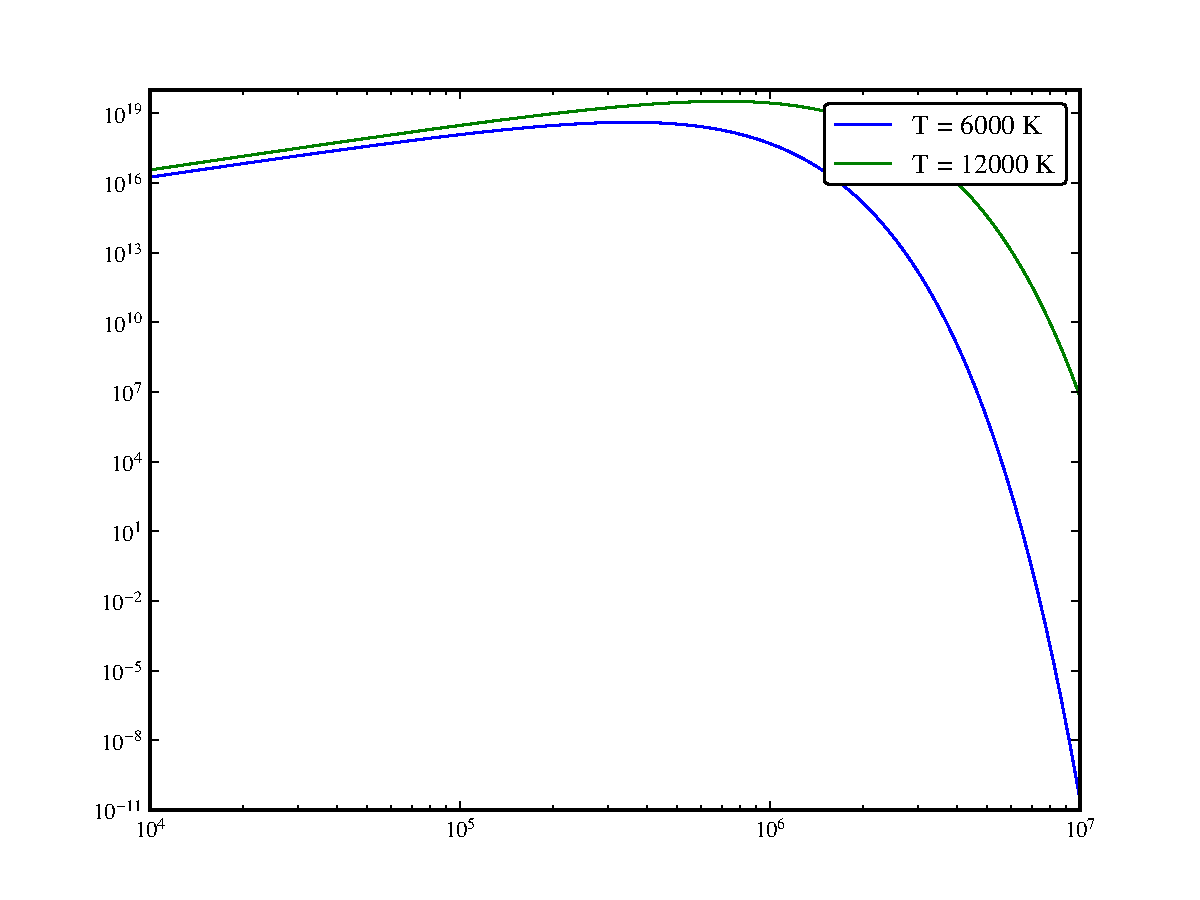
\includegraphics{functions-1.pdf}

\end{fulllineitems}

\index{grey\_body() (in module astrolyze.functions.astro\_functions)}

\begin{fulllineitems}
\phantomsection\label{functions:astrolyze.functions.astro_functions.grey_body}\pysiglinewithargsret{\code{astrolyze.functions.astro\_functions.}\bfcode{grey\_body}}{\emph{p}, \emph{x}, \emph{nu\_or\_lambda='nu'}, \emph{kappa='Kruegel'}, \emph{distance=840000.0}}{}
Calculation of the flux density in Jansky of a grey\_body under assumption
of optically thin emission.

Please see {\color{red}\bfseries{}Notes\_} below for an detailed description assumptions and
equations used.
\begin{quote}\begin{description}
\item[{Parameters }] \leavevmode
\textbf{p: list} :
\begin{quote}

List of the parameters defining a grey\_body, being Temperature {[}K{]},
column density or mass (dependent on the kappa used) and the grey\_body
slope index beta, respectively (refer to notes for more information):
\begin{quote}

p = {[}T, N, beta{]}
\end{quote}
\end{quote}

\textbf{x: float or numpy array} :
\begin{quote}

Wavelength {[}GHz{]} or frequency {[}micron{]};
specify type in nu\_or\_lambda
\end{quote}

\textbf{kappa: string} :
\begin{quote}
\begin{description}
\item[{Chooses the dust extinction coefficient to use:}] \leavevmode\begin{itemize}
\item {} 
\code{"easy"} -\textgreater{} kappa = nu\textasciicircum{}beta; tau = N * kappa

\item {} 
\code{"Kruegel"} -\textgreater{} kappa = 0.04*(nu/250Ghz)\textasciicircum{}beta;
tau = M/D\textasciicircum{}2 * kappa

\end{itemize}

\end{description}

Please refer to Notes below, for further explanation.
\end{quote}

\textbf{distance: float} :
\begin{quote}

The distance to the source that is to be modeled if kappa
\code{"Kruegel"} is used.
\end{quote}

\item[{Other Parameters}] \leavevmode
\textbf{nu\_or\_lambda: string} :
\begin{quote}

Specify whether x is a frequency $\nu$ \code{'nu'} or a wavelength
$\lambda$ \code{'lambda'}; default is \code{'nu'}. if lambda the input
converted to a frequency in {[}GHz{]}.
\end{quote}

\end{description}\end{quote}
\paragraph{Notes}

The general equation for a grey\_body is:
\begin{gather}
\begin{split}S(x, \tau) = (black_body(x, T)) * [1 - e^\tau] \Omega\end{split}\notag
\end{gather}
describing the flux coming from an solid angle
$\Omega$ while $\tau$ is:
\begin{gather}
\begin{split}\tau_{\nu} = \frac{ \kappa_d(\nu) * M_{dust}}{D^2 \Omega} .\end{split}\notag
\end{gather}
Here we assume optically thin emission and a source filling factor of
unity. This simplifies the equation of the grey\_body to:
\begin{gather}
\begin{split}S(x, \tau) = \tau * (black_body(x, T))\end{split}\notag
\end{gather}
This script supports two versions of the dust extinction coefficient.::
A simple version without a lot of physics put into, kappa = \code{'easy'}
which defaults to the following grey\_body equation:
\begin{gather}
\begin{split}S(x, \tau) = N * x^{\beta} * black_body(x,T) ,\end{split}\notag
\end{gather}
with N being a column density scaling factor.

The second version, kappa = \code{'Kruegel'} uses the dust extinction
coefficient reported in {[}KS{]} which renders the used equation to:
\begin{gather}
\begin{split}\kappa = 0.04 * (\frac{x\,[GHz]}{250\,GHz})^{\beta}\end{split}\notag\\\begin{split}S_{\nu} = M[kg] / D^2[m^2] * \kappa * black_body(x,T) .\end{split}\notag
\end{gather}\paragraph{References}

{\hyperref[functions:ks]{{[}KS{]}}}
\paragraph{Examples}

The same examples as for {\hyperref[functions:astrolyze.functions.astro_functions.black_body]{\code{black\_body()}}} apply.

\end{fulllineitems}

\index{multi\_component\_grey\_body() (in module astrolyze.functions.astro\_functions)}

\begin{fulllineitems}
\phantomsection\label{functions:astrolyze.functions.astro_functions.multi_component_grey_body}\pysiglinewithargsret{\code{astrolyze.functions.astro\_functions.}\bfcode{multi\_component\_grey\_body}}{\emph{pMulti}, \emph{x}, \emph{nu\_or\_lambda='nu'}, \emph{kappa='Kruegel'}}{}
Combines multiple grey\_body functions and returns the flux density in
Jansky for the input frequency/wavelenght.
\begin{description}
\item[{pMulti: nested lists}] \leavevmode
Similar to p from
\code{functions.astroFunctions.grey\_body()} but the three entries are
lists, i.e.::
pMulti = {[}{[}T1, T2, T3, ...Tn{]}, {[}N1, N2, N3,...Nn{]}, {[}beta{]}{]}

\item[{x: float or numpy array}] \leavevmode
frequency {[}micron{]} (or wavelenght \textbf{Not maintained}, specify type in
nu\_or\_lambda)

\end{description}
\begin{quote}\begin{description}
\item[{Returns }] \leavevmode
\textbf{sum(snu): float} :
\begin{quote}

All dust components summed.
\end{quote}

\textbf{snu:} :
\begin{quote}

A list with the fluxes of the individual components.
\end{quote}

\end{description}\end{quote}


\strong{See Also:}


{\hyperref[functions:astrolyze.functions.astro_functions.black_body]{\code{black\_body}}}, {\hyperref[functions:astrolyze.functions.astro_functions.grey_body]{\code{grey\_body}}}


\paragraph{Notes}

Only one common beta for all components can be used. May be expanded to
mutliple betas if needed.
\paragraph{Examples}

Same as for black\_body, but all returned grey\_bodies may be plotted.

\end{fulllineitems}

\index{grey\_body\_fit() (in module astrolyze.functions.astro\_functions)}

\begin{fulllineitems}
\phantomsection\label{functions:astrolyze.functions.astro_functions.grey_body_fit}\pysiglinewithargsret{\code{astrolyze.functions.astro\_functions.}\bfcode{grey\_body\_fit}}{\emph{data}, \emph{start\_parameter}, \emph{nu\_or\_lambda='nu'}, \emph{fit\_beta=False}, \emph{fix\_temperature=False}, \emph{rawChiSq=None}, \emph{kappa='Kruegel'}, \emph{residuals=False}, \emph{iterations=1000000000.0}}{}
This function fits a multi component grey body model to an observed SED for
the optical thin case.
\begin{quote}\begin{description}
\item[{Parameters }] \leavevmode
\textbf{data: array} :
\begin{quote}

The obseved data. Array of shape(3, x) first row has to be the X values
(Frequency in {[}GHz{]}) of the measurements, second row the Y values
(Flux {[}Jy{]}), and the third row  the Z values the errors on the
fluxes i.e.:
\begin{quote}

data = array({[}{[}X1, X2, X3, ...{]}, {[}Y1, Y2, Y3,...{]}, {[}Z1, Z2,
Z3, ...{]}{]})
\end{quote}
\end{quote}

\textbf{start\_parameter: array} :
\begin{quote}

Array of a first guess of the parameters of the grey\_body components.
The number of components is arbitrary
\begin{quote}

start\_parameter = {[}{[}T1, T2, T3,...{]}, {[}N1, N2, N3, ...{]}, beta{]}
\end{quote}
\end{quote}

\textbf{fit\_beta: True or False} :
\begin{quote}

If True Beta is allowed to vary. Default is False.
\end{quote}

\textbf{fix\_temperature: True or False} :
\begin{quote}

If True the Temperature is fixed allowed to vary.
\end{quote}

\textbf{rawChiSq:} :
\begin{quote}

if None the function gives the reduced chisq Value. If True the
function gives chisq without dividing it by the dof
\end{quote}

\item[{Returns }] \leavevmode
\textbf{p2: list} :
\begin{quote}

The final grey\_body parameters that reduce the least squares for the
given dataset.
\end{quote}

\textbf{chisq/rawChiSq:} :
\begin{quote}
\begin{description}
\item[{chisq is reduced chisq with degrees of freedom:}] \leavevmode
dof= \#dataPoints-\#freeFitParameters-1

\end{description}
\end{quote}

\item[{Other Parameters}] \leavevmode
\textbf{nu\_or\_lambda: string} :
\begin{quote}

Specify whether x is a frequency $\nu$ \code{'nu'} or
a wavelenght $\lambda$ \code{'lambda'}; default is \code{'nu'}.::
\textbf{Don't} use \code{'lambda'} as this part of the
{\hyperref[functions:astrolyze.functions.astro_functions.grey_body]{\code{grey\_body()}}} is not up-to-date.
\end{quote}

\end{description}\end{quote}


\strong{See Also:}

\begin{description}
\item[{\code{scipy.optimize.leastsq}}] \leavevmode
This function is used to perform the least squares

\end{description}

\code{fit.}, {\hyperref[functions:astrolyze.functions.astro_functions.multi_component_grey_body]{\code{multi\_component\_grey\_body}}}, {\hyperref[functions:astrolyze.functions.astro_functions.grey_body]{\code{grey\_body}}}, {\hyperref[functions:astrolyze.functions.astro_functions.black_body]{\code{black\_body}}}, \code{be}


\paragraph{Notes}

A one component fit has four free parameters if beta is allowed to vary or
three if beta is fixed (one more than parameters to fit). Each additional
component adds two more free paramters to fit.
Assure that:
\begin{quote}

number of data points \textgreater{} number of free parameters.
\end{quote}

\end{fulllineitems}

\index{LTIR() (in module astrolyze.functions.astro\_functions)}

\begin{fulllineitems}
\phantomsection\label{functions:astrolyze.functions.astro_functions.LTIR}\pysiglinewithargsret{\code{astrolyze.functions.astro\_functions.}\bfcode{LTIR}}{\emph{p2}, \emph{kappa='Kruegel'}, \emph{xmin=3.0}, \emph{xmax=1100.0}, \emph{beamConv=True}, \emph{distance=847000.0}, \emph{unit='JyB'}}{}
Integration of a multi-component greybody model.
\begin{quote}\begin{description}
\item[{Parameters }] \leavevmode
\textbf{p2: list} :
\begin{quote}

The parameters defining the multi-component greybody model. Same format
as p in
\code{astrolyze.functions.astroFunctions.multi\_component\_grey\_body()}
\end{quote}

\textbf{kappa: string} :
\begin{quote}

The dust extinction coefficient used to describe the greybodies. See:
py:func:\emph{grey\_body}
\end{quote}

\textbf{xmin, xmax: float} :
\begin{quote}

The integration range in units of micron. Defaults to 3 -- 110 micron.
The definition of LTIR from {[}DA{]}
\end{quote}

\textbf{beamConv: True or False} :
\begin{quote}

For units in Lsun the code is not well written. Hardcoded conversion
between an 28'' and 40'' beam. !! CHANGE !!
\end{quote}

\textbf{unit: string} :
\begin{quote}

If \code{'Lsun'} the returned integrated flux is in units of solar
luminosities (erg s\textasciicircum{}-1). For this a distance is needed. If \code{'JyB'}
the units are Jy/beam; distance is not used.
\end{quote}

\end{description}\end{quote}
\paragraph{Notes}

Needs some work to be generally usable. For units in Jy/beam the code seems
to be safe.
\paragraph{References}

{\hyperref[functions:da]{{[}DA{]}}}

\end{fulllineitems}

\index{generate\_monte\_carlo\_data\_sed() (in module astrolyze.functions.astro\_functions)}

\begin{fulllineitems}
\phantomsection\label{functions:astrolyze.functions.astro_functions.generate_monte_carlo_data_sed}\pysiglinewithargsret{\code{astrolyze.functions.astro\_functions.}\bfcode{generate\_monte\_carlo\_data\_sed}}{\emph{data}}{}
MonteCarlo Simulation of a set of flux measurements, assuming that the
measurement data follows a gauss distribution.

This function makes use of the \code{random.gauss()} function to generate a
data point from a gauss distribution, that has a mean equal to the Flux
measurement and a standard deviation correponding to the error of the
measurement.
\begin{quote}\begin{description}
\item[{Parameters }] \leavevmode
\textbf{data: array} :
\begin{quote}
\begin{description}
\item[{Same format as in grey\_body\_fit function:}] \leavevmode
data= {[}{[}x1, x2, x3, ...{]}{[}y1, y2, y3, ...{]}{[}z1, z2, z3, ...{]}{]}

\end{description}

with x = wavelenght/frequency, y = flux, z = error on flux.
\end{quote}

\item[{Returns }] \leavevmode
\textbf{newData: array in same format as data.} :
\begin{quote}

The monte carlo simulated measurement.
\end{quote}

\end{description}\end{quote}


\strong{See Also:}


\code{random.gauss}



\end{fulllineitems}

\index{grey\_body\_monte\_carlo() (in module astrolyze.functions.astro\_functions)}

\begin{fulllineitems}
\phantomsection\label{functions:astrolyze.functions.astro_functions.grey_body_monte_carlo}\pysiglinewithargsret{\code{astrolyze.functions.astro\_functions.}\bfcode{grey\_body\_monte\_carlo}}{\emph{p}, \emph{data}, \emph{iterations}}{}
Function to evaluate the errors in the parameters fitted with the
grey\_body\_fit function.

It uses Monte Carlo Simulated data (from
{\hyperref[functions:astrolyze.functions.astro_functions.generate_monte_carlo_data_sed]{\code{generate\_monte\_carlo\_data\_sed()}}}) and performs a fit to this new data
giving back the results of the fit parameters.
\begin{quote}\begin{description}
\item[{Parameters }] \leavevmode
\textbf{p: list} :
\begin{quote}

The parameters defining the multi component grey\_body model to be
fitted. Same format as p in {\hyperref[functions:astrolyze.functions.astro_functions.multi_component_grey_body]{\code{multi\_component\_grey\_body()}}}
\end{quote}

\textbf{data: array} :
\begin{quote}

The actual measured data of the SED, same format as for
\code{grey\_body\_fitFunction()}
\end{quote}

\textbf{iterations: int} :
\begin{quote}

Number of times new data is generated and fitted.
\end{quote}

\item[{Returns }] \leavevmode
\textbf{string:} :
\begin{quote}

Containing the mean, standard deviation of the fit parameters, ready
to print out.
\end{quote}

\textbf{betaTlist: List of all fit results. Name misleading since it may not} :
\begin{quote}

include the beta.
\end{quote}

\end{description}\end{quote}

\end{fulllineitems}

\index{line() (in module astrolyze.functions.astro\_functions)}

\begin{fulllineitems}
\phantomsection\label{functions:astrolyze.functions.astro_functions.line}\pysiglinewithargsret{\code{astrolyze.functions.astro\_functions.}\bfcode{line}}{\emph{p}, \emph{x}}{}
Line \emph{y = m*x + b} equation. Returns y value at point x.
\begin{quote}\begin{description}
\item[{Parameters }] \leavevmode
\textbf{p: list} :
\begin{quote}

Contains the slope and the y-axis intersection of the line {[}m, b{]}.
\end{quote}

\item[{Returns }] \leavevmode
\textbf{y: value of y corresponding to x.} :

\end{description}\end{quote}

\end{fulllineitems}

\index{anti\_line() (in module astrolyze.functions.astro\_functions)}

\begin{fulllineitems}
\phantomsection\label{functions:astrolyze.functions.astro_functions.anti_line}\pysiglinewithargsret{\code{astrolyze.functions.astro\_functions.}\bfcode{anti\_line}}{\emph{p}, \emph{y}}{}
Inverse of a line returning the x value corresponding to a y value, i.e.
\emph{x = y/m - b}.
\begin{quote}\begin{description}
\item[{Parameters }] \leavevmode
\textbf{p: list} :
\begin{quote}

Contains the slope and the y-axis intersection of the line {[}m, b{]}.
\end{quote}

\item[{Returns }] \leavevmode
\textbf{y: value of x corresponding to y.} :

\end{description}\end{quote}

\end{fulllineitems}

\index{linear\_error\_function() (in module astrolyze.functions.astro\_functions)}

\begin{fulllineitems}
\phantomsection\label{functions:astrolyze.functions.astro_functions.linear_error_function}\pysiglinewithargsret{\code{astrolyze.functions.astro\_functions.}\bfcode{linear\_error\_function}}{\emph{p}, \emph{x}, \emph{y}, \emph{y\_error}, \emph{x\_error}}{}
Error function, i.e. residual from the measured value, which has to be
minimised in the least square fit taking X and Y Error into account.
\begin{quote}\begin{description}
\item[{Parameters }] \leavevmode
\textbf{p: list} :
\begin{quote}

Same as in {\hyperref[functions:astrolyze.functions.astro_functions.line]{\code{line()}}} and {\hyperref[functions:astrolyze.functions.astro_functions.anti_line]{\code{anti\_line()}}}.
\end{quote}

\textbf{x: float or list} :
\begin{quote}

x measurements. Data.
\end{quote}

\textbf{y: float or list} :
\begin{quote}

y measurements. Data.
\end{quote}

\textbf{x\_error: float or list} :
\begin{quote}

The x measurment errors.
\end{quote}

\textbf{y\_error: float or list} :
\begin{quote}

The y measurment errors.
\end{quote}

\end{description}\end{quote}

\end{fulllineitems}

\index{line\_fit() (in module astrolyze.functions.astro\_functions)}

\begin{fulllineitems}
\phantomsection\label{functions:astrolyze.functions.astro_functions.line_fit}\pysiglinewithargsret{\code{astrolyze.functions.astro\_functions.}\bfcode{line\_fit}}{\emph{p}, \emph{x}, \emph{y}, \emph{y\_error}, \emph{x\_error=False}, \emph{iterations=10000}}{}
Linear Fit to data, taking either errors in y or both in x and y into
account.
\begin{quote}\begin{description}
\item[{Parameters }] \leavevmode
\textbf{p: list} :
\begin{quote}

Containg slope (m) and y-axis intersection (b) p={[}m, b{]}. Same as in
{\hyperref[functions:astrolyze.functions.astro_functions.line]{\code{line()}}} and \code{antiline()}.
\end{quote}

\textbf{x: float or list} :
\begin{quote}

x measurements. Data.
\end{quote}

\textbf{y: float or list} :
\begin{quote}

y measurements. Data.
\end{quote}

\textbf{y\_error: float or list} :
\begin{quote}

The y measurment errors.
\end{quote}

\textbf{x\_error: float or list} :
\begin{quote}

The x measurment errors. If unset only errors in y are taken into
account.
\end{quote}

\end{description}\end{quote}

\end{fulllineitems}

\index{analytic\_linear\_fit() (in module astrolyze.functions.astro\_functions)}

\begin{fulllineitems}
\phantomsection\label{functions:astrolyze.functions.astro_functions.analytic_linear_fit}\pysiglinewithargsret{\code{astrolyze.functions.astro\_functions.}\bfcode{analytic\_linear\_fit}}{\emph{x}, \emph{y}, \emph{x\_error}, \emph{y\_error}}{}
This function resembles the analytical solution following chaper 8 from
{[}TA{]}.
\begin{quote}\begin{description}
\item[{Parameters }] \leavevmode
\textbf{x: float or list} :
\begin{quote}

x measurements. Data.
\end{quote}

\textbf{y: float or list} :
\begin{quote}

y measurements. Data.
\end{quote}

\textbf{y\_error: float or list} :
\begin{quote}

The y measurment errors.
\end{quote}

\textbf{x\_error: float or list} :
\begin{quote}

The x measurment errors. If unset only errors in y are taken into
account.
\end{quote}

\end{description}\end{quote}
\paragraph{Notes}

Without errors the following holds:
\begin{gather}
\begin{split}y = A + B x\end{split}\notag\\\begin{split}A = \frac{\Sigma(x^2) \cdot \Sigma(y) - \Sigma(x) \cdot
\Sigma(x \cdot y)}{\Delta}\end{split}\notag\\\begin{split}B = N \frac{\Sigma(x \cdot y) - \Sigma (x) \cdot \Sigma(y)}{\Delta}\end{split}\notag\\\begin{split}\Delta = N \cdot \Sigma(x^2) - (\Sigma(x))^2\end{split}\notag
\end{gather}
\begin{notice}{warning}{Warning:}
This has to be checked.
\end{notice}
\paragraph{References}

{\hyperref[functions:ta]{{[}TA{]}}}

\end{fulllineitems}

\index{generate\_monte\_carlo\_data\_line() (in module astrolyze.functions.astro\_functions)}

\begin{fulllineitems}
\phantomsection\label{functions:astrolyze.functions.astro_functions.generate_monte_carlo_data_line}\pysiglinewithargsret{\code{astrolyze.functions.astro\_functions.}\bfcode{generate\_monte\_carlo\_data\_line}}{\emph{data}, \emph{errors}}{}
This function makes a Monte Carlo Simulation of a data Set of measurements
it uses the random.gauss() function to generate a data point
from a gauss distribution, that has a mean equal to the measurement
and its standard deviation corresonding to the error of the measurement.
\begin{quote}\begin{description}
\item[{Parameters }] \leavevmode
\textbf{data: list} :
\begin{quote}

A list of original measurements.
\end{quote}

\textbf{errors: list} :
\begin{quote}

A list of the corresponding errors.
\end{quote}

\item[{Returns }] \leavevmode
\textbf{newData: array in same format as data.} :
\begin{quote}

The monte carlo simulated measurement.
\end{quote}

\end{description}\end{quote}


\strong{See Also:}


\code{random.gauss}



\end{fulllineitems}

\index{line\_monte\_carlo() (in module astrolyze.functions.astro\_functions)}

\begin{fulllineitems}
\phantomsection\label{functions:astrolyze.functions.astro_functions.line_monte_carlo}\pysiglinewithargsret{\code{astrolyze.functions.astro\_functions.}\bfcode{line\_monte\_carlo}}{\emph{p}, \emph{x}, \emph{y}, \emph{x\_error}, \emph{y\_error}, \emph{iterations}, \emph{fitIterations=1000000000.0}}{}
Gererate an estimate of the errors of the fitted parameters determined by
the {\hyperref[functions:astrolyze.functions.astro_functions.line_fit]{\code{line\_fit()}}} function.
\begin{quote}\begin{description}
\item[{Parameters }] \leavevmode
\textbf{p: list} :
\begin{quote}

Containg slope (m) and y-axis intersection (b) p={[}m, b{]}. Same as in
{\hyperref[functions:astrolyze.functions.astro_functions.line]{\code{line()}}} and \code{antiline()}.
\end{quote}

\textbf{x: float or list} :
\begin{quote}

x measurements. Data.
\end{quote}

\textbf{y: float or list} :
\begin{quote}

y measurements. Data.
\end{quote}

\textbf{y\_error: float or list} :
\begin{quote}

The y measurment errors.
\end{quote}

\textbf{x\_error: float or list} :
\begin{quote}

The x measurment errors. If unset only errors in y are taken into
account.
\end{quote}

\item[{Returns }] \leavevmode
\textbf{string: A string containing the results.} :

\textbf{BList: A list containing the fittet y-Axis intersections.} :

\textbf{MList: A list containing the fitted slopes.} :

\textbf{chisqList: A list with the chisq values.} :

\textbf{resultArray: Array with the mean and the standard deviations of} :
\begin{quote}

slopes and y-axis intersections, i.e. {[}mean(M), std(M), mean(B),
std(B){]}
\end{quote}

\end{description}\end{quote}


\strong{See Also:}


{\hyperref[functions:astrolyze.functions.astro_functions.grey_body_fit]{\code{grey\_body\_fit}}}, {\hyperref[functions:astrolyze.functions.astro_functions.generate_monte_carlo_data_line]{\code{generate\_monte\_carlo\_data\_line}}}



\end{fulllineitems}

\index{gauss1D() (in module astrolyze.functions.astro\_functions)}

\begin{fulllineitems}
\phantomsection\label{functions:astrolyze.functions.astro_functions.gauss1D}\pysiglinewithargsret{\code{astrolyze.functions.astro\_functions.}\bfcode{gauss1D}}{\emph{x}, \emph{fwhm}, \emph{offset=0}, \emph{amplitude=1}}{}
Calulcates 1D Gaussian.
\begin{quote}\begin{description}
\item[{Parameters }] \leavevmode
\textbf{x: float or numpy.ndarray} :
\begin{quote}

the x-axis value/values where the Gaussian is to be caluclated.
\end{quote}

\textbf{fwhm: float} :
\begin{quote}

The width of the Gaussian.
\end{quote}

\textbf{offset:} :
\begin{quote}

The offset in x direction from 0. Default is 0.
\end{quote}

\textbf{amplitude:} :
\begin{quote}

The height of the Gaussian. Default is 1.
\end{quote}

\item[{Returns }] \leavevmode
\textbf{gauss: float or np.ndarray} :
\begin{quote}

The y value for the specified Gaussian distribution evaluated at x.
\end{quote}

\end{description}\end{quote}
\paragraph{Notes}

The function used to describe the Gaussian is:
\begin{gather}
\begin{split}f = \frac{1}{fwhm * sqrt(2 * \pi)} * e^{-1/2 (\frac{x-x0}{fwhm})^2}\end{split}\notag
\end{gather}
\end{fulllineitems}

\index{gauss2D() (in module astrolyze.functions.astro\_functions)}

\begin{fulllineitems}
\phantomsection\label{functions:astrolyze.functions.astro_functions.gauss2D}\pysiglinewithargsret{\code{astrolyze.functions.astro\_functions.}\bfcode{gauss2D}}{\emph{x}, \emph{y}, \emph{major}, \emph{minor}, \emph{pa=0}, \emph{xOffset=0}, \emph{yOffset=0}, \emph{amplitude=1}}{}
Calculates a 2D Gaussian at position x y.
\begin{quote}\begin{description}
\item[{Parameters }] \leavevmode
\textbf{x: float or numpy.ndarray} :
\begin{quote}

the x-axis value/values where the Gaussian is to be caluclated.
\end{quote}

\textbf{y: float or numpy.ndarray} :
\begin{quote}

the y-axis value/values where the Gaussian is to be calculated.
\end{quote}

\textbf{major, minor: float} :
\begin{quote}

The fwhm of the Gaussian in x and y direction.
\end{quote}

\textbf{pa: float} :
\begin{quote}

The position angle of the Gaussian in degrees. Default is 0.
\end{quote}

\textbf{xOffset, yOffset:} :
\begin{quote}

The offset in x and y direction from 0. Default is 0.
\end{quote}

\textbf{amplitude:} :
\begin{quote}

The height of the Gaussian. Default is 1.
\end{quote}

\item[{Returns }] \leavevmode
\textbf{gauss: float or np.ndarray} :
\begin{quote}

The y value for the specified Gaussian distribution evaluated at x.
\end{quote}

\end{description}\end{quote}
\paragraph{Notes}

The function used to describe the Gaussian is :
\begin{gather}
\begin{split}f = (amplitude * exp (-1 (a*(x-xOffset)^2 + 2*b*(x-xOffset)*(y-yOffset)
    + c*(y-yOffset)^2)))\end{split}\notag
\end{gather}
where:
\begin{gather}
\begin{split}a = cos(pa)**2/(2*major**2) + sin(pa)**2/(2*minor**2) \\
b = (-1*sin(2*pa)/(4*major**2))+(sin(2*pa)/(4*minor**2)) \\
c = sin(pa)**2/(2*major**2) + cos(pa)**2/(2*minor**2) \\\end{split}\notag
\end{gather}
\end{fulllineitems}

\index{degrees\_to\_equatorial() (in module astrolyze.functions.astro\_functions)}

\begin{fulllineitems}
\phantomsection\label{functions:astrolyze.functions.astro_functions.degrees_to_equatorial}\pysiglinewithargsret{\code{astrolyze.functions.astro\_functions.}\bfcode{degrees\_to\_equatorial}}{\emph{degrees}}{}
Converts RA, DEC coordinates in degrees to equatorial notation.
\begin{quote}\begin{description}
\item[{Parameters }] \leavevmode
\textbf{degrees: list} :
\begin{quote}

The coordinates in degrees in the format of: {[}23.4825, 30.717222{]}
\end{quote}

\item[{Returns }] \leavevmode
\textbf{equatorial: list} :
\begin{quote}

The coordinates in equatorial notation, e.g.
corresponding {[}`1:33:55.80', `+30:43:2.00'{]}.
\end{quote}

\end{description}\end{quote}

\end{fulllineitems}

\index{equatorial\_to\_degrees() (in module astrolyze.functions.astro\_functions)}

\begin{fulllineitems}
\phantomsection\label{functions:astrolyze.functions.astro_functions.equatorial_to_degrees}\pysiglinewithargsret{\code{astrolyze.functions.astro\_functions.}\bfcode{equatorial\_to\_degrees}}{\emph{equatorial}}{}
Converts RA, DEC coordinates in equatorial notation to degrees.
\begin{quote}\begin{description}
\item[{Parameters }] \leavevmode
\textbf{equatorial: list} :
\begin{quote}

The coordinates in degress in equatorial notation, e.g.
{[}`1:33:55.80', `+30:43:2.00'{]}
\end{quote}

\item[{Returns }] \leavevmode
\textbf{degrees: list} :
\begin{quote}

The coordinates in degreees, e.g. {[}23.4825, 30.717222{]}.
\end{quote}

\item[{Raises }] \leavevmode
\textbf{SystemExit} :
\begin{quote}

If \code{equatorial} is not a list of strings in the above format.
\end{quote}

\end{description}\end{quote}

\end{fulllineitems}

\index{calc\_offset() (in module astrolyze.functions.astro\_functions)}

\begin{fulllineitems}
\phantomsection\label{functions:astrolyze.functions.astro_functions.calc_offset}\pysiglinewithargsret{\code{astrolyze.functions.astro\_functions.}\bfcode{calc\_offset}}{\emph{central\_coordinate}, \emph{offset\_coordinate}, \emph{angle=0}, \emph{output\_unit='farcsec'}}{}
Calculates the offset between two coordinates.
\begin{quote}\begin{description}
\item[{Parameters }] \leavevmode
\textbf{central\_coordinate: list} :
\begin{quote}

The reference coordinate in degrees or equatorial.
\end{quote}

\textbf{offset\_coordinate: list} :
\begin{quote}

The second coordinate, the offset will be with rescpect to
central\_coordinate.
\end{quote}

\textbf{angle: float} :
\begin{quote}

The angle in degrees, allowing rotated systems.
\end{quote}

\item[{Returns }] \leavevmode
\textbf{rotated\_offset: list} :
\begin{quote}

The offsets, rotated only if angle given.
\end{quote}

\end{description}\end{quote}
\paragraph{Notes}

This functions includes a correction of the RA offset with declination:

\end{fulllineitems}

\index{rotation\_2d() (in module astrolyze.functions.astro\_functions)}

\begin{fulllineitems}
\phantomsection\label{functions:astrolyze.functions.astro_functions.rotation_2d}\pysiglinewithargsret{\code{astrolyze.functions.astro\_functions.}\bfcode{rotation\_2d}}{\emph{coordinate}, \emph{angle}}{}
Implementation of the rotation matrix in two dimensions.
\begin{quote}\begin{description}
\item[{Parameters }] \leavevmode
\textbf{coordinates: list of floats} :
\begin{quote}

Coordinates in the unrotated system {[}x, y{]}.
\end{quote}

\textbf{angle: float} :
\begin{quote}

The rotation angle
\end{quote}

\item[{Returns }] \leavevmode
\textbf{{[}x\_rotated, y\_rotated{]}: list of floats} :
\begin{quote}

Coordinates in the rotated system.
\end{quote}

\end{description}\end{quote}

\end{fulllineitems}



\section{units}
\label{functions:units}
Constant unit conversions availabe in this module are:

\begin{Verbatim}[commandchars=\\\{\}]
\PYG{c}{\PYGZsh{} Constant conversion factors.}
\PYG{c}{\PYGZsh{}==============\textgreater{} Approved !!! \textless{}==========================}
\PYG{n}{WattToErgs}    \PYG{o}{=} \PYG{l+m+mf}{1e7}  \PYG{c}{\PYGZsh{} 1W = 1e7 erg/s}
\PYG{n}{ErgsToWatt}    \PYG{o}{=} \PYG{l+m+mf}{1e-7}  \PYG{c}{\PYGZsh{} 1W = 1e-7 erg/s}
\PYG{n}{JanskyToWatt}  \PYG{o}{=} \PYG{l+m+mf}{1e-26}  \PYG{c}{\PYGZsh{} 1Jy = 1e-26 W/m2/Hz}
\PYG{n}{WattToJansky}  \PYG{o}{=} \PYG{l+m+mf}{1e26}  \PYG{c}{\PYGZsh{} 1W  = 1 Jy * m2 * Hz}
\PYG{n}{ErgsToJansky\PYGZus{}cm}  \PYG{o}{=} \PYG{l+m+mf}{1e23}  \PYG{c}{\PYGZsh{} 1 erg/s =  1e23 Jy * cm2 * Hz * s}
\PYG{n}{JanskyToErgs\PYGZus{}cm}  \PYG{o}{=} \PYG{l+m+mf}{1e-23}  \PYG{c}{\PYGZsh{} 1 Jy = 1e-23 erg/s/cm2/Hz}
\end{Verbatim}
\phantomsection\label{functions:module-astrolyze.functions.units}\index{astrolyze.functions.units (module)}\index{WmToKkms() (in module astrolyze.functions.units)}

\begin{fulllineitems}
\phantomsection\label{functions:astrolyze.functions.units.WmToKkms}\pysiglinewithargsret{\code{astrolyze.functions.units.}\bfcode{WmToKkms}}{\emph{x}, \emph{resolution=0}, \emph{sterad=False}, \emph{ToKKms=False}, \emph{m2\_or\_cm2='m'}, \emph{nu\_or\_lambda='nu'}}{}
Conversion between W/m2 and K km/s.
\begin{quote}\begin{description}
\item[{Parameters }] \leavevmode
\textbf{x: float} :
\begin{quote}

wavelenght/frequency {[}GHZ{]}.
\end{quote}

\textbf{resolution: float} :

\textbf{ToKKms: True or False} :
\begin{quote}

Direction of the conversion.
\end{quote}

\textbf{sterad: True or False} :
\begin{quote}

If False convert from per beam to per sterad.
\end{quote}

\textbf{m2\_or\_cm2: string} :
\begin{quote}

Choose if conversion to/from W m-2 oder W cm-2. \code{'m2'} or \code{'cm2'}.
\end{quote}

\item[{Returns }] \leavevmode
\textbf{factor: float} :
\begin{quote}

The conversion factor.
\end{quote}

\end{description}\end{quote}

\end{fulllineitems}

\index{ergToKkms() (in module astrolyze.functions.units)}

\begin{fulllineitems}
\phantomsection\label{functions:astrolyze.functions.units.ergToKkms}\pysiglinewithargsret{\code{astrolyze.functions.units.}\bfcode{ergToKkms}}{\emph{x}, \emph{toErg=False}, \emph{nu\_or\_lambda='nu'}}{}
Conversion between ergs/cm2/s/sr and K km/s.
\begin{quote}\begin{description}
\item[{Parameters }] \leavevmode
\textbf{x: float} :
\begin{quote}

wavelenght/frequency {[}GHZ{]},
\end{quote}

\textbf{toErg: True or False} :
\begin{quote}

True converts the other direction, i.e. from K km/s to ergs/cm2/s/sr.
\end{quote}

\textbf{nu\_or\_lambda: string} :
\begin{quote}

Choose type of x: frequency = \code{'nu'} or wavelenght = \code{'lambda'}.
\end{quote}

\item[{Returns }] \leavevmode
\textbf{factor: float} :
\begin{quote}

The conversion factor.
\end{quote}

\end{description}\end{quote}
\paragraph{Notes}

Approved.

\end{fulllineitems}

\index{Int2Lum() (in module astrolyze.functions.units)}

\begin{fulllineitems}
\phantomsection\label{functions:astrolyze.functions.units.Int2Lum}\pysiglinewithargsret{\code{astrolyze.functions.units.}\bfcode{Int2Lum}}{\emph{distance\_in\_pc}, \emph{cm\_or\_m='cm'}}{}
Conversion factor to calculate luminosity from intensities
by integrating over the sky 4 pi Distance\textasciicircum{}2.
\begin{quote}\begin{description}
\item[{Parameters }] \leavevmode
\textbf{distance\_in\_pc: float} :
\begin{quote}

Distance to the source in parsecs.
\end{quote}

\textbf{cm\_or\_m: string} :
\begin{quote}

Choose wether the out put is in cm\textasciicircum{}2 = \code{'cm'} or in
m\textasciicircum{}2 = \code{'m'}.
\end{quote}

\textbf{Notes} :

\textbf{-----} :

\textbf{Approved.} :

\end{description}\end{quote}

\end{fulllineitems}

\index{JyBToErgsB() (in module astrolyze.functions.units)}

\begin{fulllineitems}
\phantomsection\label{functions:astrolyze.functions.units.JyBToErgsB}\pysiglinewithargsret{\code{astrolyze.functions.units.}\bfcode{JyBToErgsB}}{\emph{input\_flux}, \emph{distance}, \emph{wavelength}, \emph{invert=False}, \emph{map\_use=False}}{}
Conversion between Jy/beam and ergs/beam.
\begin{quote}\begin{description}
\item[{Parameters }] \leavevmode
\textbf{input\_flux: float} :
\begin{quote}

Flux to be converted in Jy/beam
\end{quote}

\textbf{distance: float} :
\begin{quote}

Distance to the source in parsec.
\end{quote}

\textbf{wavelength: float} :
\begin{quote}

Wavelength $\lambda$ in $\mu m$.
\end{quote}

\textbf{map\_use:} :

\item[{Returns }] \leavevmode
\textbf{The conversion factor (map\_use = true) or the already converted flux} :

\textbf{(map\_use = False).} :

\textbf{r} :

\end{description}\end{quote}

\end{fulllineitems}

\index{JyBToWM2Kpc2() (in module astrolyze.functions.units)}

\begin{fulllineitems}
\phantomsection\label{functions:astrolyze.functions.units.JyBToWM2Kpc2}\pysiglinewithargsret{\code{astrolyze.functions.units.}\bfcode{JyBToWM2Kpc2}}{\emph{input\_flux}, \emph{distance}, \emph{major}, \emph{minor}, \emph{wavelength}, \emph{invert=False}, \emph{map\_use=False}}{}
Conversion between Jy/beam and W m\textasciicircum{}-2 kpc\textasciicircum{}-2
\begin{quote}\begin{description}
\item[{Parameters }] \leavevmode
\textbf{input\_flux:  float} :
\begin{quote}

Flux to be converted.
\end{quote}

\textbf{distance: float} :
\begin{quote}

Distance to source in parsec.
\end{quote}

\textbf{major: float} :
\begin{quote}

Major Axis Beam (arcsec).
\end{quote}

\textbf{minor: float} :
\begin{quote}

Minor Axis Beam(arcsec).
\end{quote}

\textbf{wavelength: float} :
\begin{quote}

Wavelenght $\lambda$ in $\mu m$
\end{quote}

\textbf{invert: True or False} :
\begin{quote}

Changes the direction of conversion.
\end{quote}

\item[{Returns }] \leavevmode
\textbf{float: the converted Flux.} :

\end{description}\end{quote}

\end{fulllineitems}

\index{JyBToWKpc2() (in module astrolyze.functions.units)}

\begin{fulllineitems}
\phantomsection\label{functions:astrolyze.functions.units.JyBToWKpc2}\pysiglinewithargsret{\code{astrolyze.functions.units.}\bfcode{JyBToWKpc2}}{\emph{input\_flux}, \emph{distance}, \emph{major}, \emph{minor}, \emph{wavelength}, \emph{invert=False}, \emph{map\_use=False}}{}
Conversion from JyB to W kpc\textasciicircum{}-2.
\begin{quote}\begin{description}
\item[{Parameters }] \leavevmode
\textbf{input\_flux:  float} :
\begin{quote}

Flux to be converted.
\end{quote}

\textbf{distance: float} :
\begin{quote}

Distance to source in parsec.
\end{quote}

\textbf{major: float} :
\begin{quote}

Major Axis Beam (arcsec).
\end{quote}

\textbf{minor: float} :
\begin{quote}

Minor Axis Beam(arcsec).
\end{quote}

\textbf{wavelength: float} :
\begin{quote}

Wavelenght $\lambda$ in $\mu m$.
\end{quote}

\textbf{invert: True or False} :
\begin{quote}

Changes the direction of conversion.
\end{quote}

\item[{Returns }] \leavevmode
\textbf{float: the converted Flux.} :

\end{description}\end{quote}

\end{fulllineitems}

\index{kelvin\_to\_jansky() (in module astrolyze.functions.units)}

\begin{fulllineitems}
\phantomsection\label{functions:astrolyze.functions.units.kelvin_to_jansky}\pysiglinewithargsret{\code{astrolyze.functions.units.}\bfcode{kelvin\_to\_jansky}}{\emph{x}, \emph{major}, \emph{minor}, \emph{nu\_or\_lambda='nu'}}{}
Conversion from K.km/s (Tmb) and Jy/beam.
\begin{quote}\begin{description}
\item[{Parameters }] \leavevmode
\textbf{x: float} :
\begin{quote}

wavelength/frequency {[}GHZ{]},
\end{quote}

\textbf{major: float} :
\begin{quote}

Major Axis Beam (arcsec),
\end{quote}

\textbf{minor: float} :
\begin{quote}

Minor Axis Beam(arcsec),
\end{quote}

\textbf{nu\_or\_lambda: string} :
\begin{quote}

Choose type of x: frequency = \code{'nu'} or wavelength = \code{'lambda'}.
\end{quote}

\end{description}\end{quote}
\paragraph{Notes}

This function has been compared with the Time estimator from the
{[}GILDAS{]} package ASTRO and yields the same conversion factors.
\paragraph{References}

{\hyperref[manual:gildas]{{[}GILDAS{]}}}

\end{fulllineitems}

\index{jansky\_to\_kelvin() (in module astrolyze.functions.units)}

\begin{fulllineitems}
\phantomsection\label{functions:astrolyze.functions.units.jansky_to_kelvin}\pysiglinewithargsret{\code{astrolyze.functions.units.}\bfcode{jansky\_to\_kelvin}}{\emph{x}, \emph{major}, \emph{minor}, \emph{nu\_or\_lambda='nu'}}{}
Conversion from Jy/beam to K.km/s (Tmb).
\begin{quote}\begin{description}
\item[{Parameters }] \leavevmode
\textbf{x: float} :
\begin{quote}

wavelength/frequency {[}GHZ{]},
\end{quote}

\textbf{major: float} :
\begin{quote}

Major Axis Beam (arcsec).
\end{quote}

\textbf{minor: float} :
\begin{quote}

Minor Axis Beam(arcsec).
\end{quote}

\textbf{nu\_or\_lambda: string} :
\begin{quote}

Choose type of x: frequency = \code{'nu'} or wavelength = \code{'lambda'}.
\end{quote}

\end{description}\end{quote}
\paragraph{Notes}

Same as {\hyperref[functions:astrolyze.functions.units.kelvin_to_jansky]{\code{kelvin\_to\_jansky()}}}

\end{fulllineitems}



\section{constants}
\label{functions:constants}
\begin{Verbatim}[commandchars=\\\{\}]
\PYG{c}{\PYGZsh{} Natural Constants}
\PYG{n}{c} \PYG{o}{=} \PYG{l+m+mf}{299792458.}  \PYG{c}{\PYGZsh{} Speed of light [m]}
\PYG{n}{c\PYGZus{}in\PYGZus{}cm} \PYG{o}{=} \PYG{n}{c} \PYG{o}{*} \PYG{l+m+mf}{1e2}  \PYG{c}{\PYGZsh{} Speed of light [cm]}
\PYG{n}{h} \PYG{o}{=} \PYG{l+m+mf}{6.62606896e-34}  \PYG{c}{\PYGZsh{} Plancks constant [Js]}
\PYG{n}{k} \PYG{o}{=} \PYG{l+m+mf}{1.3806503e-23}  \PYG{c}{\PYGZsh{} Boltzman constant [m\PYGZca{}2 kg s\PYGZca{}-1 K\PYGZca{}-1]}
\PYG{n}{tBG} \PYG{o}{=} \PYG{l+m+mf}{2.7}  \PYG{c}{\PYGZsh{} Cosmic Microwave Background Temperature in [K]}
\PYG{n}{e} \PYG{o}{=} \PYG{l+m+mf}{2.7182818284}  \PYG{c}{\PYGZsh{} Eulers number }

\PYG{c}{\PYGZsh{} Natural Constants in cgs units.}
\PYG{n}{k\PYGZus{}CGS} \PYG{o}{=} \PYG{l+m+mf}{1.3806503e-16}  \PYG{c}{\PYGZsh{} Boltzman constant [cm\PYGZca{}2 g s\PYGZca{}-1 K\PYGZca{}-1]}
\PYG{n}{h\PYGZus{}CGS} \PYG{o}{=} \PYG{l+m+mf}{6.62606896e-27}  \PYG{c}{\PYGZsh{} Plancks constant [Js]}
\PYG{n}{c\PYGZus{}CGS} \PYG{o}{=} \PYG{l+m+mf}{2.99792458e10}  \PYG{c}{\PYGZsh{} Speed of light [cm]}

\PYG{c}{\PYGZsh{} Conversion of distances}
\PYG{n}{parsec\PYGZus{}in\PYGZus{}m\PYGZus{}1} \PYG{o}{=} \PYG{l+m+mf}{3.08568025e16}
\PYG{n}{parsec\PYGZus{}in\PYGZus{}m} \PYG{o}{=} \PYG{l+m+mf}{3.085e16}  \PYG{c}{\PYGZsh{} parsec in m}
\PYG{n}{parsec\PYGZus{}in\PYGZus{}cm} \PYG{o}{=} \PYG{l+m+mf}{3.08568025e18}  \PYG{c}{\PYGZsh{} parsec in cm}
\PYG{n}{km\PYGZus{}in\PYGZus{}cm} \PYG{o}{=} \PYG{l+m+mf}{1e5}

\PYG{c}{\PYGZsh{} Masses}
\PYG{n}{m\PYGZus{}sun} \PYG{o}{=} \PYG{l+m+mf}{1.9891e30}  \PYG{c}{\PYGZsh{} [kg]}
\PYG{n}{m\PYGZus{}proton} \PYG{o}{=} \PYG{l+m+mf}{1.672621637e-27}  \PYG{c}{\PYGZsh{} [kg]}

\PYG{c}{\PYGZsh{} Gauss constants}
\PYG{c}{\PYGZsh{} GaussArea/(height*FWHM)}
\PYG{n}{gauss\PYGZus{}constant} \PYG{o}{=} \PYG{l+m+mf}{1.064467}

\PYG{c}{\PYGZsh{} Luminosities }
\PYG{n}{LsunW} \PYG{o}{=} \PYG{l+m+mf}{3.846e26}  \PYG{c}{\PYGZsh{} Watts}
\PYG{n}{Lsunergs} \PYG{o}{=} \PYG{l+m+mf}{3.846e26}\PYG{o}{*}\PYG{l+m+mf}{1e7}  \PYG{c}{\PYGZsh{} erg/s}
\PYG{n}{debye\PYGZus{}to\PYGZus{}EsuCm} \PYG{o}{=} \PYG{l+m+mf}{1.e-18}  \PYG{c}{\PYGZsh{} Change from debye to esu/cm}

\PYG{c}{\PYGZsh{} Angle Conversions}
\PYG{n}{a2r} \PYG{o}{=} \PYG{l+m+mf}{4.848e-6}  \PYG{c}{\PYGZsh{} arcsec to radian}
\PYG{n}{a2d} \PYG{o}{=} \PYG{l+m+mf}{1.}\PYG{o}{/}\PYG{l+m+mi}{60}\PYG{o}{/}\PYG{l+m+mi}{60}  \PYG{c}{\PYGZsh{} arcsec to degree}
\PYG{n}{r2d} \PYG{o}{=} \PYG{l+m+mf}{180.}\PYG{o}{/}\PYG{n}{math}\PYG{o}{.}\PYG{n}{pi}  \PYG{c}{\PYGZsh{} radian to degree}
\end{Verbatim}


\chapter{Indices and tables}
\label{index:indices-and-tables}\begin{itemize}
\item {} 
\emph{genindex}

\item {} 
\emph{modindex}

\item {} 
\emph{search}

\end{itemize}

\begin{thebibliography}{Doktorarbeit}
\bibitem[GILDAS]{GILDAS}{\phantomsection\label{manual:gildas} 
www.iram.fr/IRAMFR/GILDAS
}
\bibitem[MIRIAD]{MIRIAD}{\phantomsection\label{manual:miriad} 
www.atnf.csiro.au/computing/sof tware/miriad/taskindex.html
}
\bibitem[Doktorarbeit]{Doktorarbeit}{\phantomsection\label{lte:doktorarbeit} 
add reference
}
\bibitem[KS]{KS}{\phantomsection\label{functions:ks} 
Kruegel, E. \& Siebenmorgen, R. 1994, A\&A, 288, 929
}
\bibitem[DA]{DA}{\phantomsection\label{functions:da} 
Dale et al. 2001; ApJ; 549:215-227
}
\bibitem[TA]{TA}{\phantomsection\label{functions:ta} 
``An introduction to the study of uncertainties in physical
measurement'' by John R. Taylor.
}
\bibitem[GILDAS]{GILDAS}{\phantomsection\label{functions:gildas} 
www.iram.fr/IRAMFR/GILDAS
}
\end{thebibliography}


\renewcommand{\indexname}{Python Module Index}
\begin{theindex}
\def\bigletter#1{{\Large\sffamily#1}\nopagebreak\vspace{1mm}}
\bigletter{a}
\item {\texttt{astrolyze.functions.astro\_functions}}, \pageref{functions:module-astrolyze.functions.astro_functions}
\item {\texttt{astrolyze.functions.units}}, \pageref{functions:module-astrolyze.functions.units}
\item {\texttt{astrolyze.lte.lte}}, \pageref{lte:module-astrolyze.lte.lte}
\item {\texttt{astrolyze.lte.molecule\_parameter}}, \pageref{lte:module-astrolyze.lte.molecule_parameter}
\item {\texttt{astrolyze.maps}}, \pageref{maps:module-astrolyze.maps}
\item {\texttt{astrolyze.maps.tools}}, \pageref{maps:module-astrolyze.maps.tools}
\end{theindex}
\renewcommand{\indexname}{Python Module Index}
\begin{theindex}
\def\bigletter#1{{\Large\sffamily#1}\nopagebreak\vspace{1mm}}
\bigletter{a}
\item {\texttt{astrolyze.functions.astro\_functions}}, \pageref{functions:module-astrolyze.functions.astro_functions}
\item {\texttt{astrolyze.functions.units}}, \pageref{functions:module-astrolyze.functions.units}
\item {\texttt{astrolyze.lte.lte}}, \pageref{lte:module-astrolyze.lte.lte}
\item {\texttt{astrolyze.lte.molecule\_parameter}}, \pageref{lte:module-astrolyze.lte.molecule_parameter}
\item {\texttt{astrolyze.maps}}, \pageref{maps:module-astrolyze.maps}
\item {\texttt{astrolyze.maps.tools}}, \pageref{maps:module-astrolyze.maps.tools}
\end{theindex}

\renewcommand{\indexname}{Index}
\printindex
\end{document}
